\documentclass[11pt,a4paper]{article}
\usepackage[utf8]{inputenc}
\usepackage[german]{babel}
\usepackage[T1]{fontenc}
\usepackage{amsmath}
\usepackage{amsfonts}
\usepackage{amssymb}
\usepackage{graphicx}
\usepackage[margin=1.25cm]{geometry} % Puts the same margin on all borders of the document

% Packages

\usepackage{hyperref} % Generate hyperlinks to referenced items
\usepackage{adjustbox} % Used to change parameters in \includegraphics[scale=•]{•}
\usepackage{enumitem} % Provides several options for lists
\usepackage{verbatim} % Package to use \begin{comment}
\usepackage{pdfpages} % Used to import PDF pages
\usepackage{multirow} % Allows us to have a single cell in a table span multiple rows
\usepackage{makecell} % Allows us to format multiple lines in a single cell
\usepackage{listings} % Used to type code in \begin{lstlisting}
\usepackage{xcolor}  % Gives access to coloring text
\usepackage{longtable} % Allows us to create a table over multiple pages
\usepackage{float} % Improved placement of floating items
\usepackage{pdfpages} % Used to import pdf pages
\usepackage{booktabs} % Used for horizontal lines instead of \hline



% Settings

\graphicspath{{./files/}} % Sets path for files to the files folder in the same directory

\hypersetup{
    colorlinks=false, %set true if you want colored links
    linktoc=all,     %set to all if you want both sections and subsections linked
    linkcolor=blue,  %choose some color if you want links to stand out
}


\begin{titlepage}
  \title{RO Reference Sheet} % document_name-type_of_document
  \author{Frederick Wichert}
  \date{Last Edited: \today}
\end{titlepage}


\begin{document}
	\pagenumbering{gobble}
	\maketitle
	
	\setcounter{secnumdepth}{2}
	\setcounter{tocdepth}{2}
	\tableofcontents
	
	\newpage
	\pagenumbering{arabic}
		
\section{Grundlagen der Rechnerorganisation}
	\subsection{Abstraktion}
		Durch verstecken unnötiger Details können zentrale Konzepte verständlich gemacht werden \\
		\begin{center}
			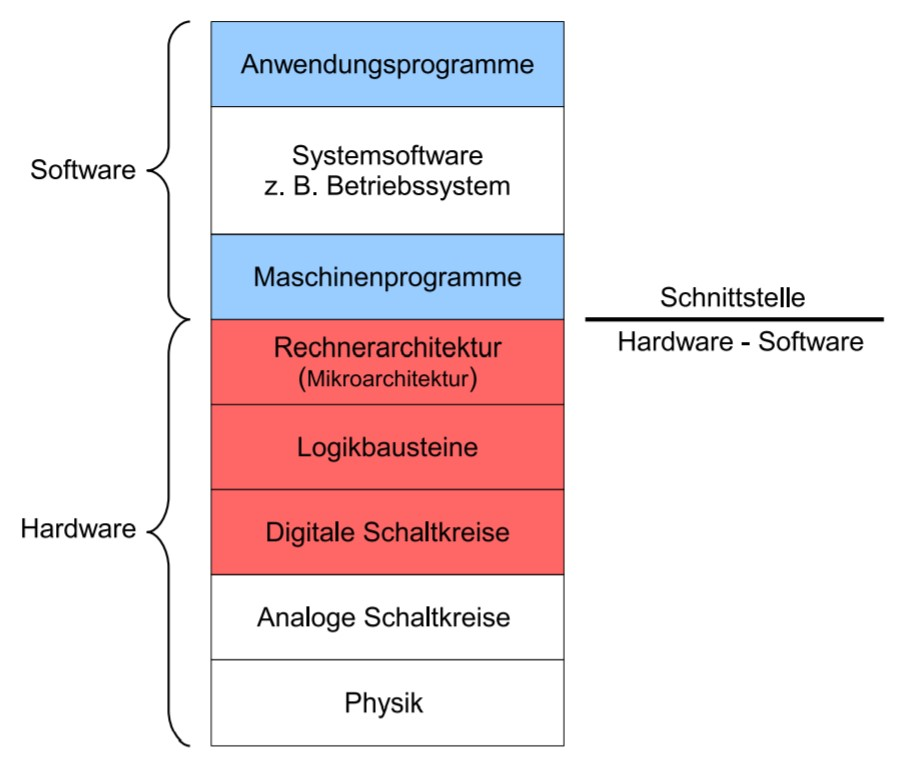
\includegraphics[scale=0.5]{SchichtenModell.jpg}
		\end{center}
		Das Schichtenmodell ist ein Beispiel für Abstraktion zur Simplifikation


	\subsection{Definition einiger Grundbegriffe}
		\paragraph{} Ein Computer \\ ist ein Datenverarbeitungssystem. Nach DIN 44300: Ein 
		Datenverarbeitungssystem ist eine Funktionseinheit zur Verarbeitung und Aufbewahrung 
		von Daten. Verarbeitung umfa\ss t die Durchführung mathematischer, umformender, übertragender und
		speichernder Operationen. \\
		Ein Rechner hat somit vier Grundfunktionen: Verarbeitung, Speichern, Umformen von Daten und Kommunizieren

		\paragraph{} Ein Paradigma \\ (Denkmuster, Musterbeispiel) ist ein übergeordnetes Prinzip.
		Es manifestiert sich in Beispielen und ist für eine ganze Teildisziplin typisch.

		\paragraph{} Ein Programmiermodell \\ bezeichnet bei Hochsprachen Grundlegende Eigenschaften
		einer Programmiersprache und bei der maschinennahen Programmierung den Registersatz eines
		Prozessors, genauer Register die durch Programme werden können sowie den Befehlssatz


	\subsection{Ein Rechnersystem aus der Praxis}
		\paragraph{} Ein Rechnersystem enthält mindestens:
		\begin{itemize}
			\item ein Prozessor (CPU) - Ausführung der Programme
			\item ein Speicher - Enthält Programme und Daten (Speichersystem)
			\item eine Möglichkeit zum Transferieren von Informationen
		\end{itemize}
		\begin{center}
			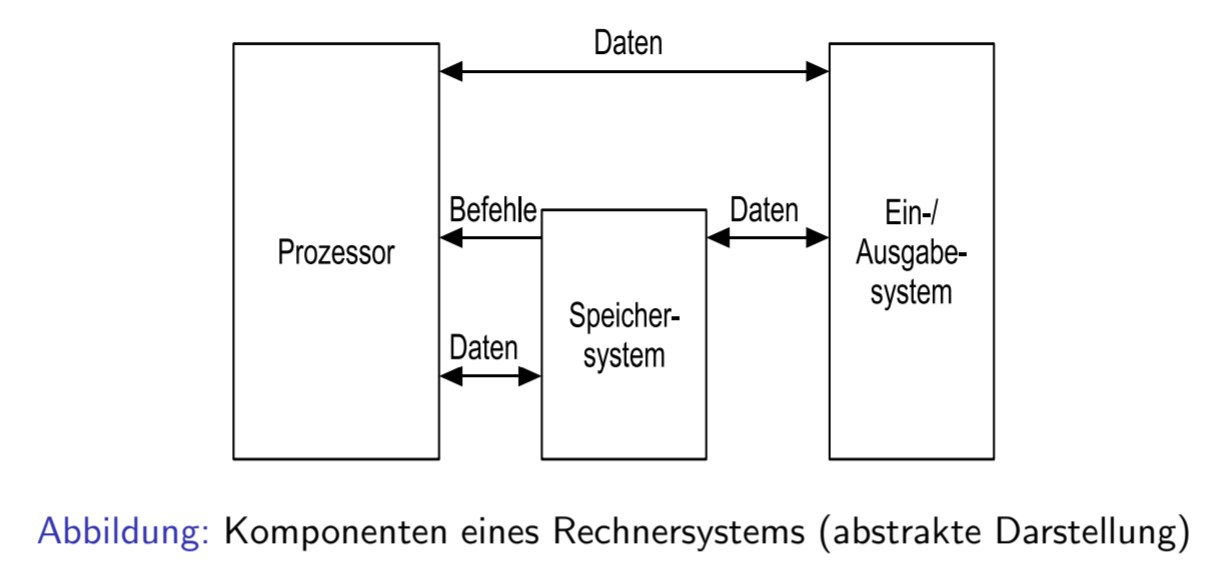
\includegraphics[scale=0.4]{KomponentenEinesRechnersystems.jpg}
			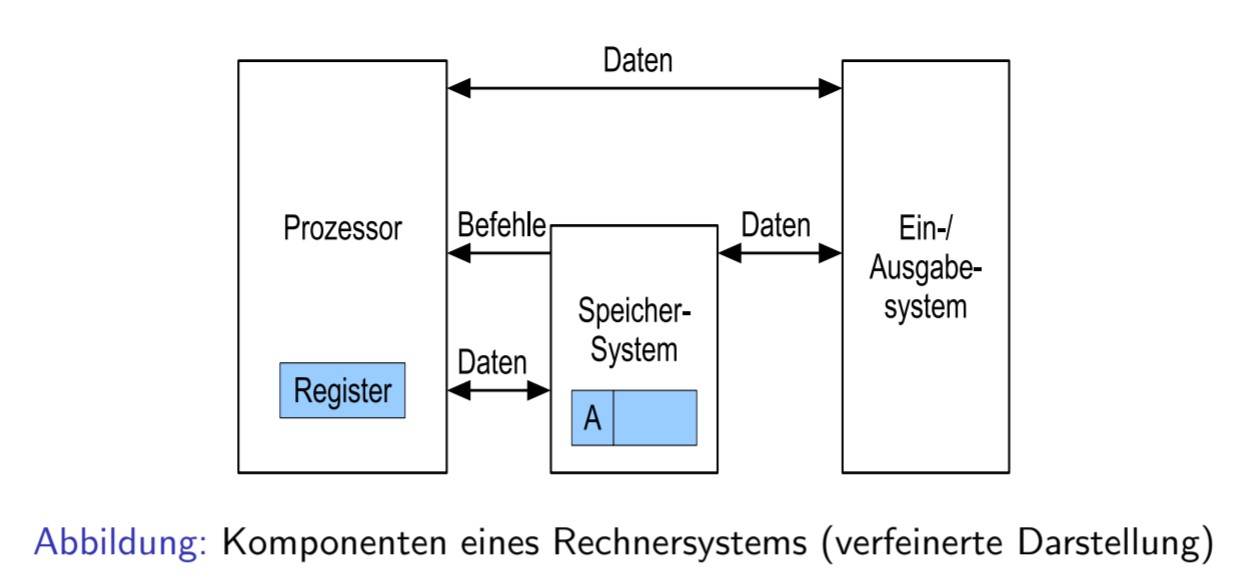
\includegraphics[scale=0.4]{KomponentenEinesRechnersystems-Verfeinert.jpg}
		\end{center}

		\paragraph{} Der Registersatz ist folgenderma\ss en Aufgebaut:
		\begin{itemize}
			\item R0
			\item R1 ... R12
			\item R13 (sp) - stack pointer (Stapelzeiger)
			\item R14 (lr) - link register (Rückkehradresse)
			\item R15 (pc) - program counter (Befählszähler)
			\item CPSR - Current Procesor Status Register (u.a. Statusflags)
		\end{itemize}
		\begin{center}
			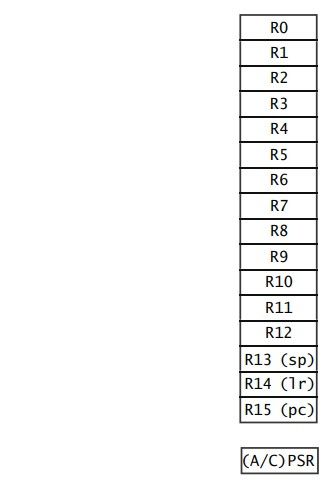
\includegraphics[scale=0.6]{Registersatz01.jpg}
			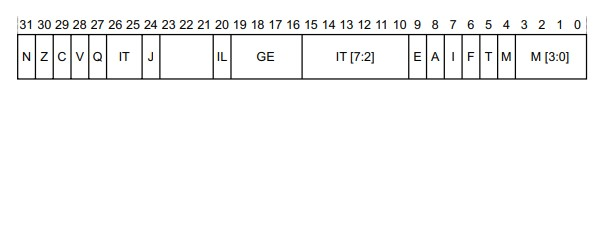
\includegraphics[scale=0.7]{Registeraufbau01.jpg}
		\end{center}


	\subsection{Speicherhierarchie}
		\paragraph{} Transparent nutzbare Speicher werden nicht direkt ansprechbar, sie werden implizit
		von einem Maschinenprogramm benutzt.
		\begin{itemize}
			\item bestimmte Register auf dem Prozessor
			\item Cache-Speicher
		\end{itemize}

		\paragraph{} Explizit nutzbare Speicher können direkt angesprochen werden.
		\begin{itemize}
			\item interner Prozessorspeicher
				\begin{itemize}
					\item schnelle Register, temporäre Nutzung (Maschinenbefehle, Daten)
					\item Direkter Zugriff durch Maschinenbefehle
					\item Technologie: Halbleiter ICs
				\end{itemize}

			\item Hauptspeicher
				\begin{itemize}
					\item relativ großer und schneller Speicher, wärhend der Ausführung
					\item Direkter Zugriff durch Maschinenbefehle
					\item Technologie: Halbleiter ICs
				\end{itemize}

			\item Sekundärspeicher
				\begin{itemize}
					\item sehr großer, sehr langsamer Speicher, permanente Speicherung
					\item Indirekter Zugriff über E/A-Programme
					\item Technologie: ICs, Megnetplatten, optische Laufwerke, Magnetbänder
				\end{itemize}
		\end{itemize}

		\begin{center}
			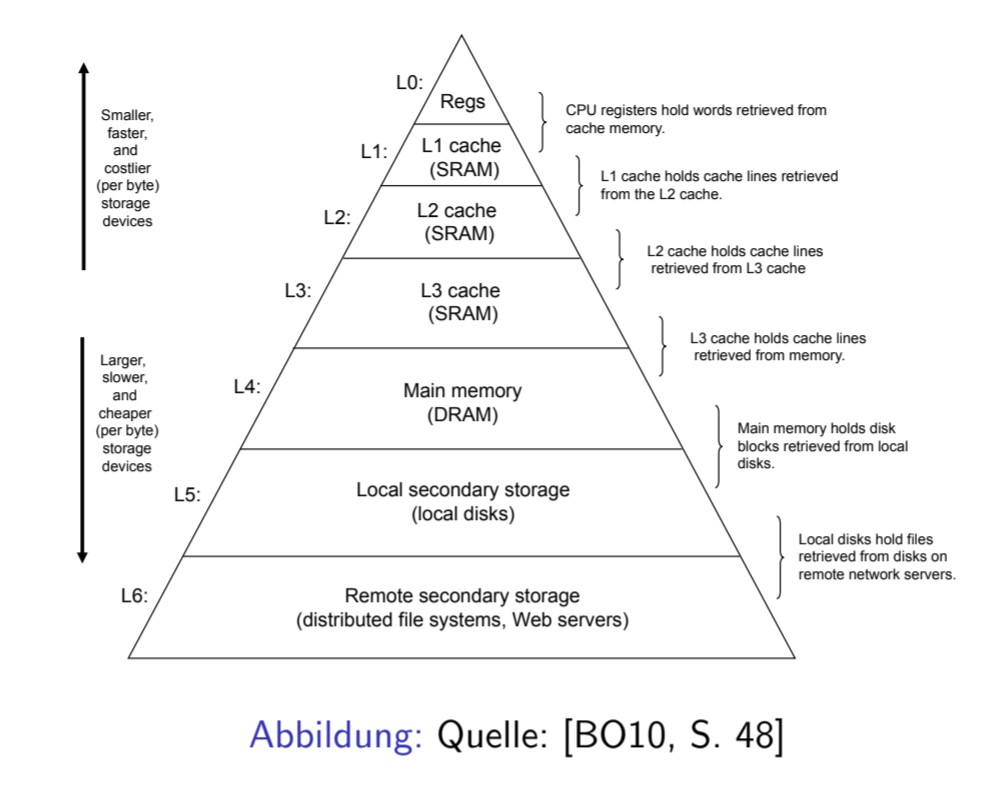
\includegraphics[scale=0.5]{SpeicherhierarchieModell.jpg}
		\end{center}



	\subsection{Speicherorganisation - Adressierung und Endian}
		\paragraph{Endian:}
		\begin{itemize}
			\item Schemata für Nummerierung von Bytes in einem Wort
		\end{itemize}
		\begin{center}
			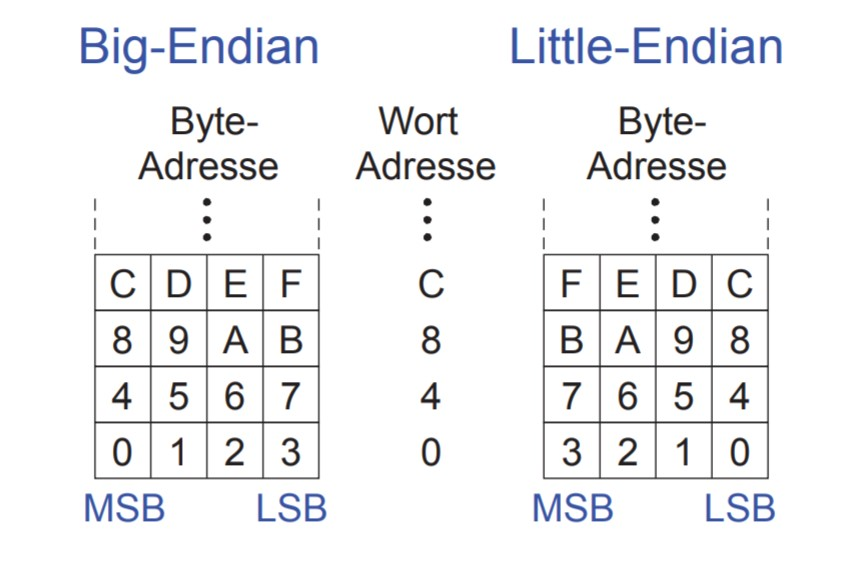
\includegraphics[scale=0.55]{LittleEndianBigEndian.jpg}
		\end{center}

		\vspace{0.7cm}

		\paragraph{Adressierung:} Die Daten passen nciht alle in 15 Register. Daher werden Daten 
		im Hauptspeicher abgelegt, dieser ist allerdings langsamer als Register. Häufig
		verwendete Daten sind daher in Registern abzulegen. Eine Kombination aus beidem
		ermöglicht optimale Laufzeit.

		\begin{itemize}
			\item ARM ist byte-adressiert, jedes byte hat eine eindeutige adresse
			\item 32.bit Wort = 4 bytes $\rightarrow$ Eine Wortadresse zeigt auf 4 bytes
			\item Adressen von Worten sind vielfache von 4
		\end{itemize}
		\begin{center}
			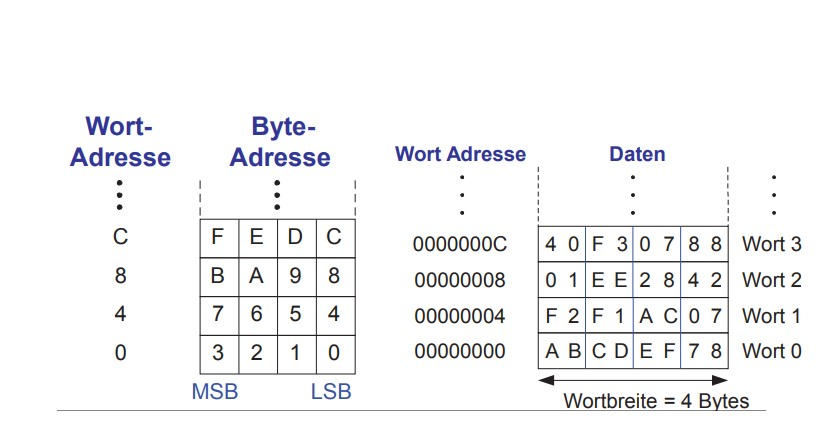
\includegraphics[scale=0.55]{ByteAdressierung01.jpg}
		\end{center}



	\subsection{Rechnersysteme - Verfeinert}
		\paragraph{Maschinenbefehle} Die Menge der Maschinenbefhele die auf einem Rechnersystem zur Verfügung stehen
		ist durch den Prozessor festgelegt. Man unterscheidet zwischen CISC (Complex Instruction Set Computer),
		z.B. Intel, und RISC (Reduced Instruction Set Computer), z.B. ARM, Maschinen. Grundsätzlich 
		enthalten alle Rechnersystem ähnliche Komponenten, aber die genaue Struktur hat Erheblichen
		Einfluss auf Kosten und Leistung. Einteilung z.B. nach n-Addressmaschinen, 2-Addressmaschinen Intel
		oder 3-Addressmaschinen ARM. Wir verwenden eine ARM Architektur. \\
		ARM = Acorn/Advanced RISC Mashines.

		\begin{center}
			Verfeinerung des Rechnersystems: \\
			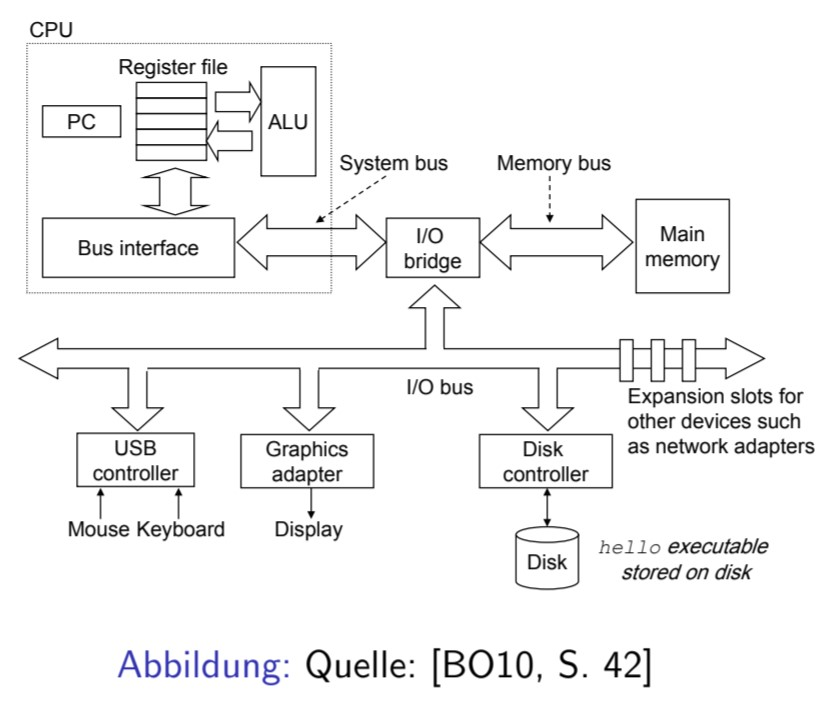
\includegraphics[scale=0.5]{RechnersystemVerfeinert.jpg}
		\end{center}

		Komponenten:
		\begin{itemize}
			\item CPU/Prozessor - führt Befehle aus dem Haptschpeicher aus
			\item ALU - Arithmetic Logic Unit
			\item PC - Programm Counter, zeigt auf nächsten Maschinenbefehl
			\item Register file - schneller Speicher für Operanden
			\item Main memory - Speichert Befehle und Daten
			\item Bus interface - Verbinden der einzelnen Komponenten
		\end{itemize}


\newpage
\section{Speicher}
	\subsection{Speicherhierarchie}
		\begin{minipage}{0.5\textwidth}
			\begin{itemize}
				\item Bisher haben wir den Speicher als lineares Feld aus Bytes
				\item Die CPU kann auf jede Speicherzelle in konstanter Zeit zugreifen
				\item In der Praxis wird eine Hierarchie mit unterschiedlichen Speichertechnologien verwendet \\
			\end{itemize}
	
			\begin{itemize}
				\item Das Lesen und Schreiben dauert gewisse Zeit, i.d.R. relativ lange im Vergleich zur Taktfrequenz
				\item Je nach Archiutektur kann das Lesen von Befehlen und Daten Parallel aus zwei Speichern erfolgen
					(Harvard) oder muss nacheinander aus einem erfolgen (Neumann)
			\end{itemize}
		\end{minipage}
		\begin{minipage}{0.45\textwidth}
			\begin{center}
				Übersicht \\
				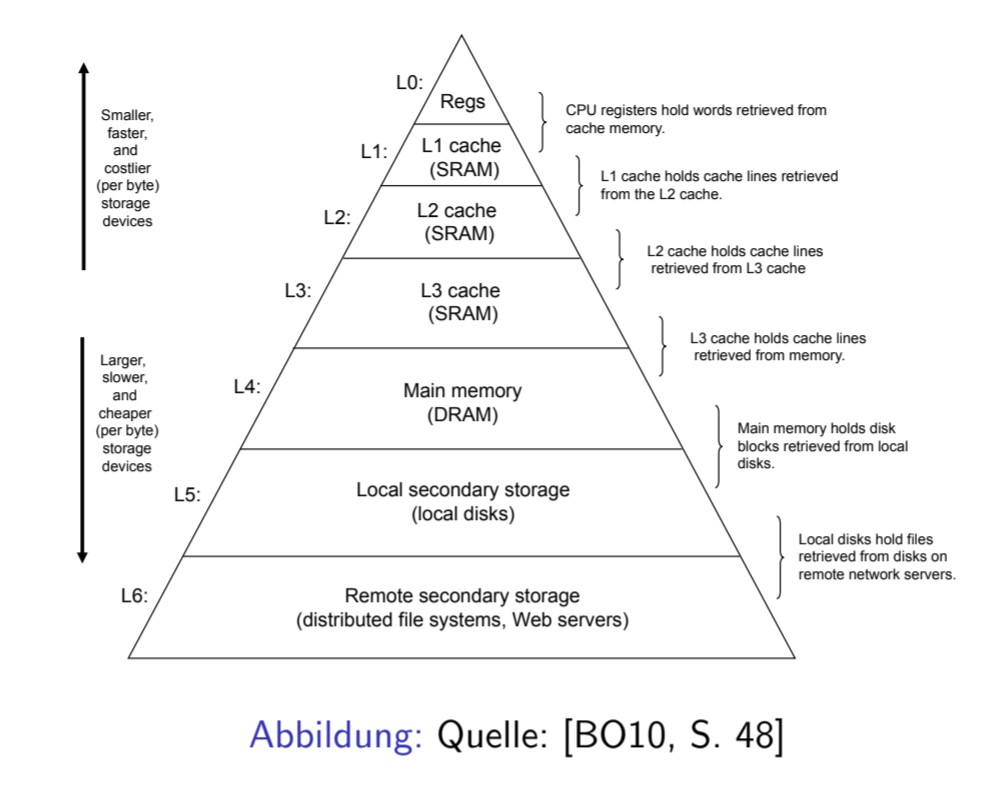
\includegraphics[scale=0.5]{SpeicherhierarchieModell.jpg}
			\end{center}
		\end{minipage}

		
		\subsubsection{Eigenschaften von Speichern}
			\begin{itemize}
				\item Kosten und Zugriffszeit
				\item Geschwindigkeit und Kapazität
				\item Zugriffsverfahren
				\item Änderbarkeit und Daten
				\item Permanenz der Daten
			\end{itemize}

		\subsubsection{Kosten und Zugriffszeit}
			\begin{itemize}
				\item in \textit{Dollar/Bit} oder \textit{Dollar/MByte}
				\item Kenngrö\ss e von Speichern
					\begin{itemize}
						\item Zugriffszeit: durchschnittliche Zeit, um ein Wort aus Speicher zu lesen
						\item Zyklsuszeit: minimal Zeit zwischen zwei Speicherzugriffen (Busprotokoll spielt eine Rolle)
						\item Bandbreite (Datenübertragungsrate): maximale Datenmenge, die pro Sekunde übertragen werden
							kann in \textit{Byte/Sec}
					\end{itemize}
			\end{itemize}


	\subsection{Speicher Kategorisierung}
		\subsubsection{Zugrissverfahren}
			\begin{itemize}
				\item Zwei Möglichkeiten
					\begin{itemize}
						\item wahlweiser Zugriff (Random Access)
						\item serieller Zugriff
					\end{itemize}
				\item Speicher mit Random Access
					\begin{itemize}
						\item Register, Cache, Hauptspeicher
					\end{itemize}
				\item Speicher mit seriellem Zugriff
					\begin{itemize}
						\item Festplatten, optische Platten, Megnetband
					\end{itemize}
			\end{itemize}

		\subsubsection{Änderbarkeit}
			\begin{itemize}
				\item Read-only:
					\begin{itemize}
						\item Speicher kann ausschlie\ss lich gelesen werden, Überschreiben ist nicht möglich
						\item ROM-Halbleiterspeicher (Read-only Memory) Inhalt wird wärhend Fabrikationsprozess
							festgelegt
					\end{itemize}
				\item Read-write:
					\begin{itemize}
						\item Inhalt kann während des Betriebs geändert werden
						\item RAM-Halbleiterspeicher (Random-access Memory) Wird als Cache- Hauptschpeicher verwendet, 
							CD-R(W), DVD
					\end{itemize}
				\item Read-mostly:
					\begin{itemize}
						\item PROM-Halbleiterspeicher oder (E)EPROM: z.B. für BIOS verwendet
					\end{itemize}
			\end{itemize}

		\subsubsection{Permanenz}
			\begin{itemize}
				\item Flüchtige Speicher (Register Hauptspeicher) vs Nicht flüchtige (ROM, PROM, EPROM Festplatte, optisches Speicherband)
				\item Flüchtige Speicher werden unterteilt:
					\begin{itemize}
						\item dynamischer Speicher: Um Informationsverlust zu vermeiden muss die Spannung periodisch
							erneuert werden (Refreshing)
						\item statische Speicher: kein Refreshing notwendig
					\end{itemize}
			\end{itemize}


	\subsection{Speichertechnologien}
		\subsubsection{Random-Access Memory (RAM)}
			\begin{itemize}
				\item Statisches RAM (SRAM) und Dynmaisches RAM (DRAM)
				\item SRAM ist schneller (deutlich teurer) als DRAM
				\item SRAM $\Rightarrow$ Cache
				\item DRAM $\Rightarrow$ Hauptspeicher
				\item Typische (vor 10 Jahren) verteilung
					\begin{itemize}
						\item 12 MB SRAM 
						\item 4 GB DRAM (heute bis zu 1.5 TB)
					\end{itemize}
			\end{itemize}
			
			\vspace{0.8cm}
			\begin{center}
				Organisation des Speichers \\
				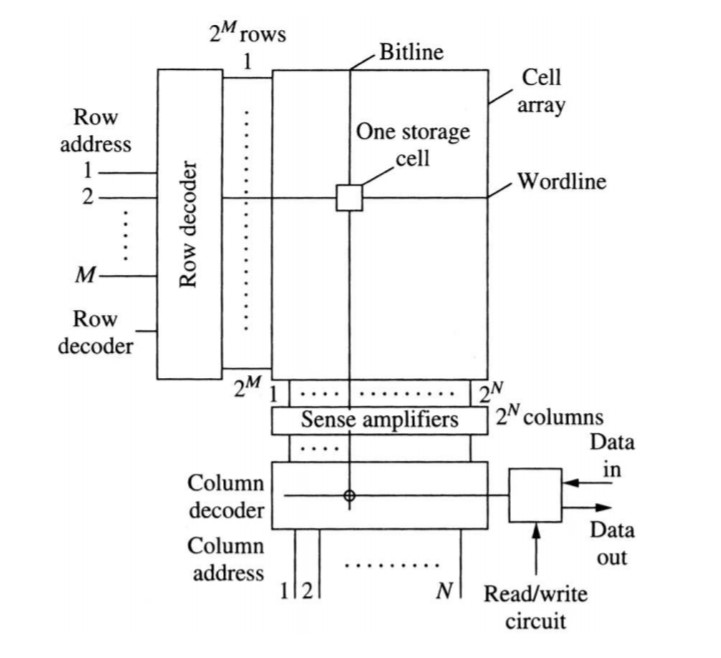
\includegraphics[scale=0.5]{RAM.jpg} \\
			\end{center}
			\begin{minipage}{0.5\textwidth}
				\centerline{Statisches RAM}
				\begin{itemize}
					\item Statisches (S)RAM speichert Informationen so lange wie die Spannungsversorgung angeschaltet ist
					\item Die gekoppelten Inverter haben zwei stabile Zustände $\Rightarrow$ Bistabile Schaltung
				\end{itemize}
				\begin{center}
					Realisierung durch Inverter - 6T Zelle, 6 Tranisistoren\\
					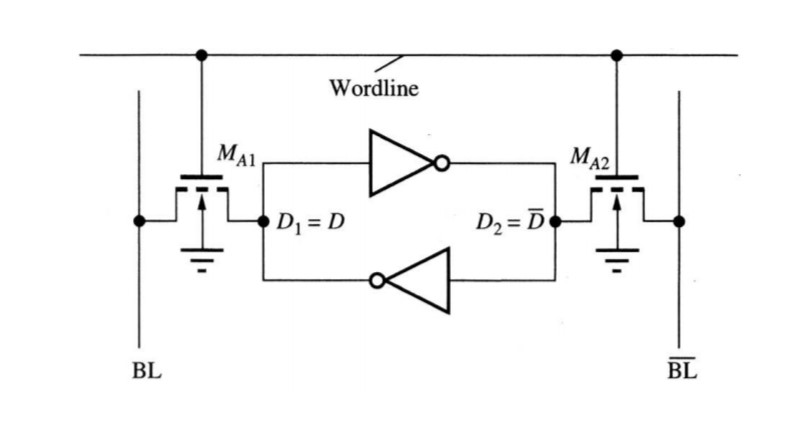
\includegraphics[scale=0.5]{SRAM01.jpg}
					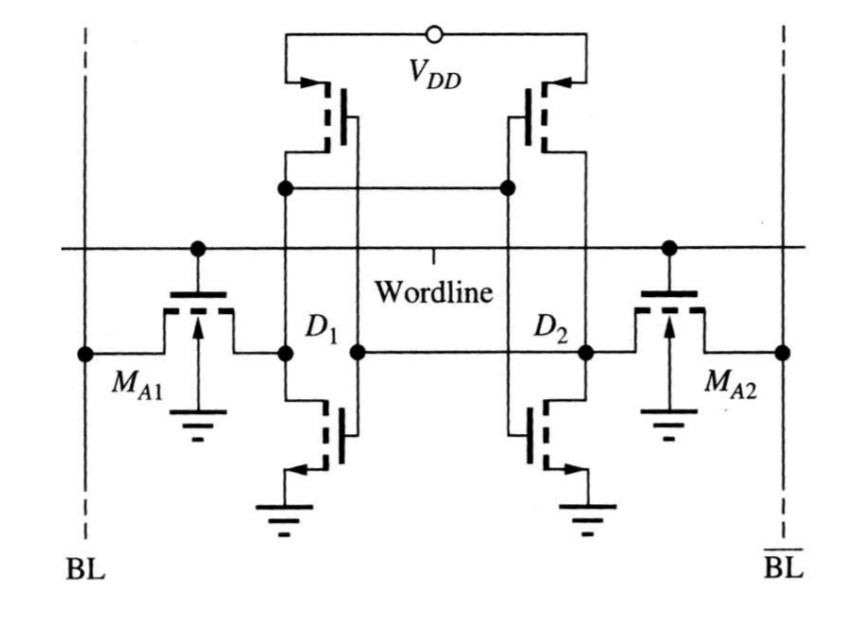
\includegraphics[scale=0.5]{SRAM02.jpg}
				\end{center}
			\end{minipage}
			\begin{minipage}{0.45\textwidth}
				\centerline{Dynamisches RAM}
				\begin{itemize}
					\item Speichert Informationen in Kondensator
					\item "1T Zelle"
					\item Der Kondensator entlädt sich und verliert damit Informationen
					\item \textbf{Refresh-Zyklus} notwendig, um Informationen aufzufrischen
				\end{itemize}
				\begin{center}
					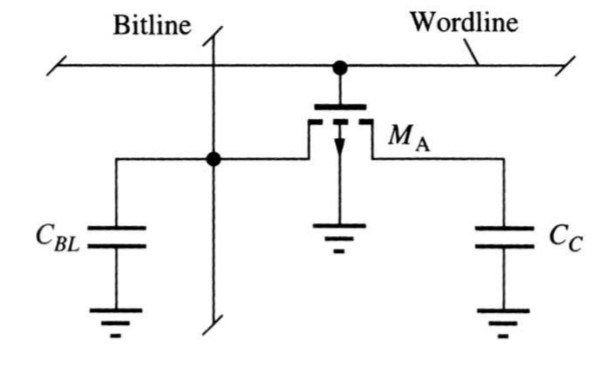
\includegraphics[scale=0.5]{DRAM01.jpg}
					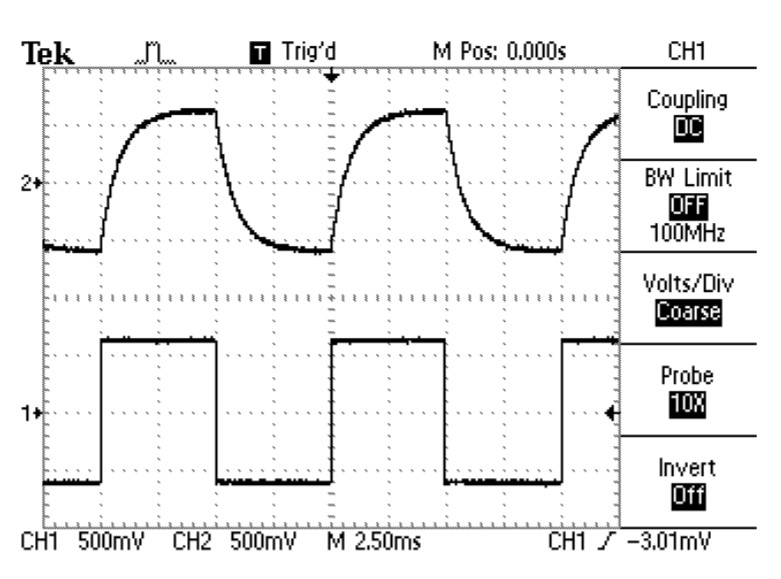
\includegraphics[scale=0.5]{DRAM02.jpg}
				\end{center}
			\end{minipage}


	\subsection{Speicherorganisation}
		\begin{itemize}
			\item Eigenschaften eines RAM-Chips sind durch zwei Grö\ss en angegeben
				\begin{itemize}
					\item Anzahl adressierbarer Plätze
					\item Breite (in Bit) jedes adressierbaren Platzes
				\end{itemize}
			\item Beispiel 256K * 1 SRAM
				\begin{itemize}
					\item 256K Einträge mit 1 Bit Breite
					\item $256K = 2^{18}$, also 18 Adresseingänge sowie ein 1 Bit Dateneingang/-ausgang
				\end{itemize}
			\end{itemize}
			\begin{minipage}{0.5\textwidth}
				\begin{itemize}
					\item 32K * 8 SRAM
						\begin{itemize}
							\item 32K Einträge mit 8 Bit Breite
							\item $32K = 2^{15}$, also 15 Adresseingänge sowie 8 Bit Dateneingang/-ausgang
						\end{itemize}
			\end{itemize}
		\end{minipage}
		\begin{minipage}{0.45\textwidth}
			\centerline{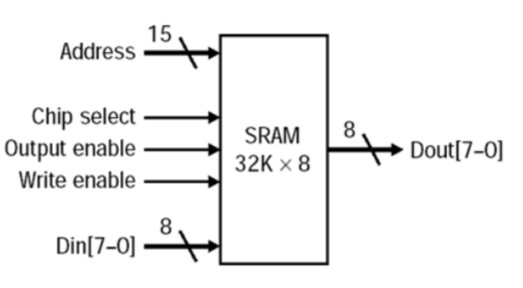
\includegraphics[scale=0.5]{32K-SRAM.jpg}}
		\end{minipage}


		\subsubsection{Darstellung: 128 Bit 16 x 8 DRAM Chips}
			\begin{minipage}{0.5\textwidth}
				Lesezugriff:
				\begin{itemize}
					\item 1. Schritt Row Address Strobe (RAS)
						\begin{itemize}
							\item Die ersten zwei Bits wählen eine Zeile (Row) aus, diese wird 
								in den internen Zeilen Speicher (internal row buffer) geladen/gespeichert
						\end{itemize}
					\item 2. Schritt Column Address Strobe (CAS)
						\begin{itemize}
							\item Die näschten zwei Bits wählen aus der gespeicherten Zeile (internal row buffer)
								die Spalte (column) aus
						\end{itemize}
				\end{itemize}
				\centerline{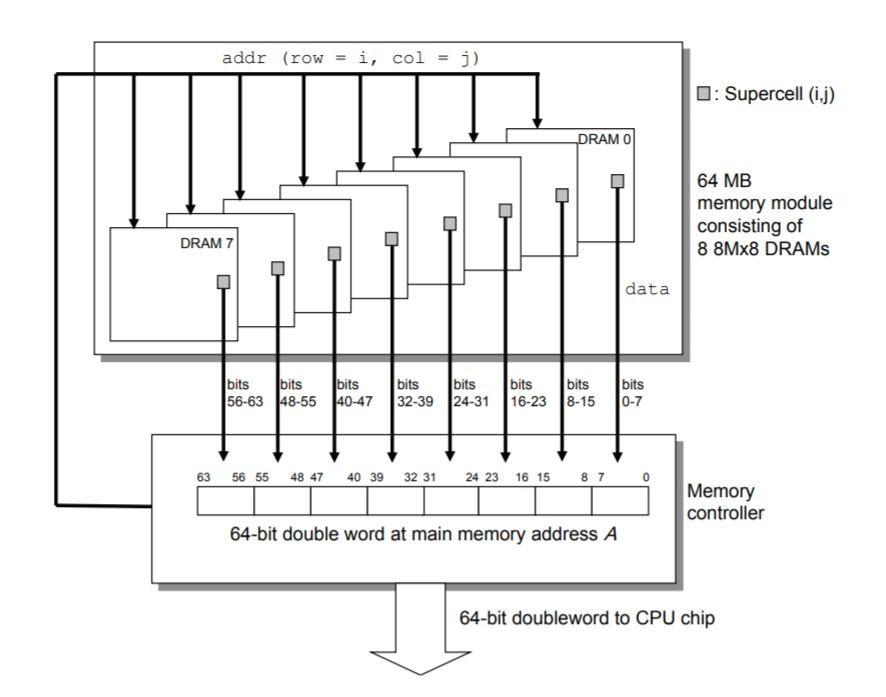
\includegraphics[scale=0.5]{VerbindungSpeichermodule.jpg}}
			\end{minipage}
			\begin{minipage}{0.45\textwidth}
				\begin{center}
					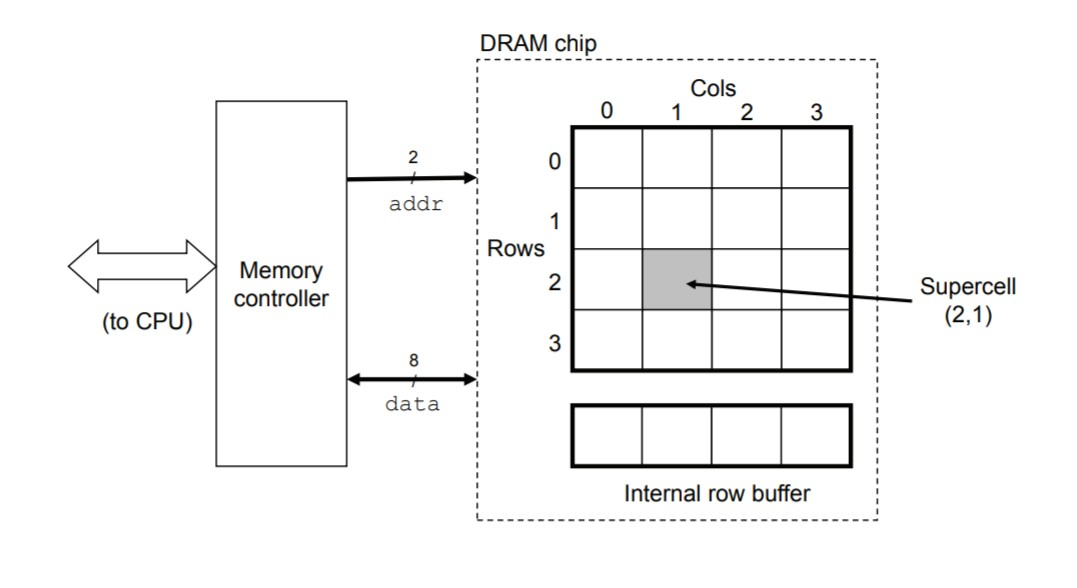
\includegraphics[scale=0.4]{DRAMChip01.jpg}
					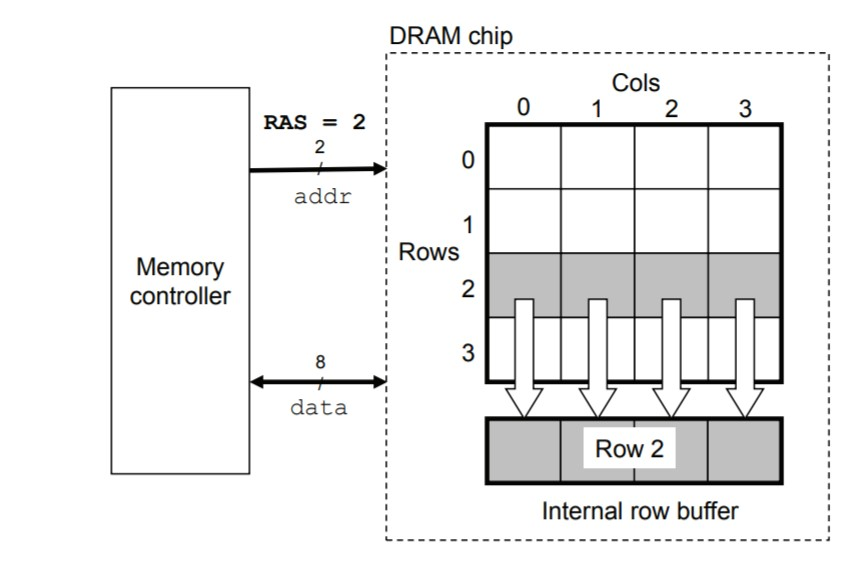
\includegraphics[scale=0.4]{DRAMChip02.jpg}
					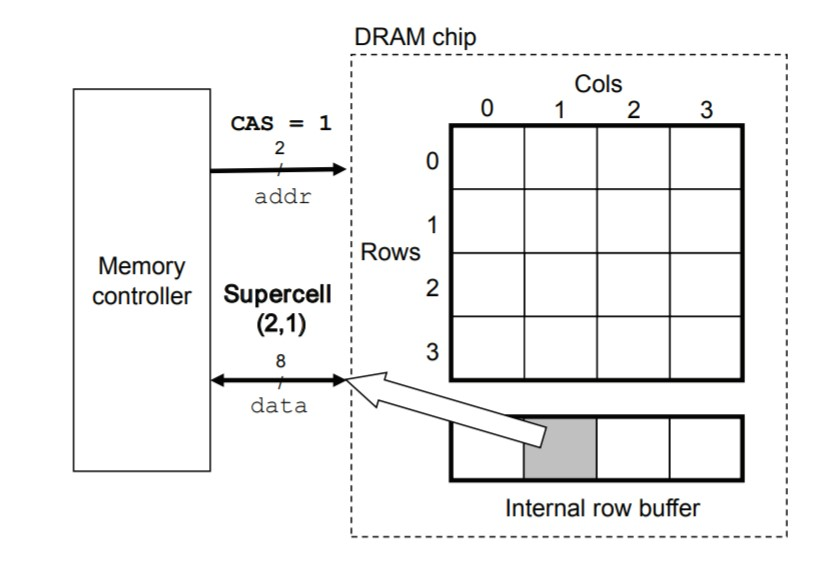
\includegraphics[scale=0.4]{DRAMChip03.jpg}
				\end{center}
			\end{minipage}

			\centerline{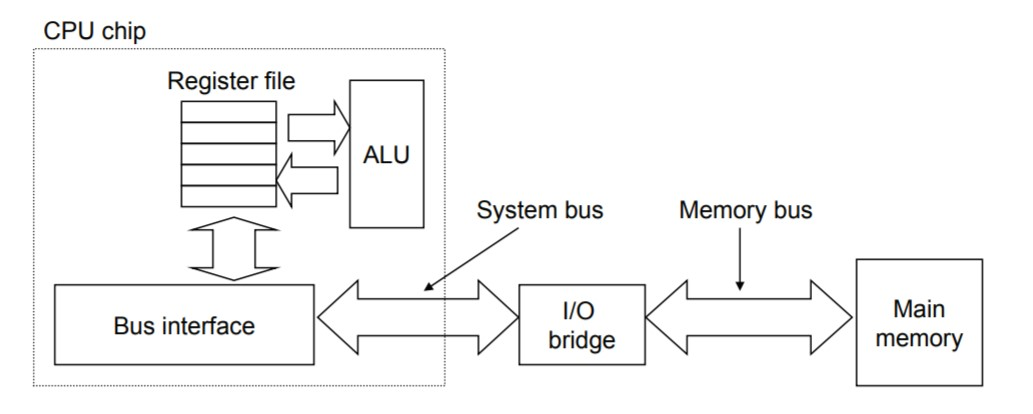
\includegraphics[scale=0.5]{CpuUndSpeicher.jpg}}


	\subsection{Lokalität}
		\begin{minipage}{0.5\textwidth}
			Das Lokalitätsprinziep stellt fest, das Programme meistens einen relativ geringen Teil des Addressraums nutzen.
		\end{minipage}
		\begin{minipage}{0.45\textwidth}
			\begin{center}
				\includegraphics[scale=0.35]{Loklaität01.jpg}
			\end{center}
		\end{minipage}

		\subsubsection{Formen der Lokalität}
			\begin{itemize}
				\item Zeitliche (temporale) Lokalität
					\begin{itemize}
						\item Nach Zugriff auf einen bestimmten Datensatz wird mit gro\ss er Wahrscheinlichkeit
							bald erneut darauf zugegriffen
						\item Beispiel: Schleifen (Indices etc.)
					\end{itemize}
				\item Räumliche Lokalität
					\begin{itemize}
						\item Nach dem Zugriff auf einen Datensatz wird mit gro\ss er Wahrscheinlichkeit auch auf 
							einen Datensatz zugegriffen, der in unmittelbarer Nähe im Speicher steht
						\item Beispiel: sequentielle Instruktionsfolge (ohne Sprünge)
						\item Beispiel: Reihungen, Matritzen
					\end{itemize}
			\end{itemize}

		\subsubsection{Vorteile}
			\begin{itemize}
				\item Gut geschriebene Programme haben eine gute Lokalität
				\item Die Anwendung des Lokalitätsprinziep hat eine enorme Auswirkung auf die Performance eines Rechnersystes (Hardware/Software)
				\item Programme mit guter Lokalität laufen schneller, als Programme mit schlechter Lokalität
				\item Zweifache Unterscheidung:
					\begin{itemize}
						\item Lokalität der Daten
						\item Lokalität der Befehle
					\end{itemize}
				\item Im Folgenden einige Beispiele für Programme mit guter und schlechter Lokalität
			\end{itemize}


		\subsubsection{Lokalität der Befehle}
			\begin{itemize}
				\item Wie die Daten sind auch Befehle im Speicher abgelegt
				\item Auch für Befehle ist also das Lokalitäts Prinziep anwendbar
				\item Für die for Schleife der Beispiele gilt eine gute räumliche Lokalität
				\item Da der Schleifenkörper wiederholt ausgeführt wird, gibt es auch eine gute zeitliche Lokalität
				\item Bei der Programmierung an das Lokalitätsprinziep denken
				\item Lokalitätsprinziep lä\ss t die Speicherhierarchie funktionieren
			\end{itemize}

		
	\subsection{Lokalität - Beispiele}
		\subsubsection{Beispiel 01}
			\begin{minipage}{0.5\textwidth}
				\begin{itemize}
					\item Elemente des Vektors werden sequentiell gelesen
					\item Beispielhaft Anordnung:
					\item Lokalität der Berechnungem:
						\begin{itemize}
							\item schlechte zeitlich Lokalität (da auf jedes Element nur einmal zugegriffen wird)
							\item gute räumliche Lokalität (da die Elemente nahe beieinander liegen)
						\end{itemize}
					\item Lokalität der Schleife:
						\begin{itemize}
							\item Schleifenindex (i) hat gute Zeitliche und räumliche Lokalität
								(da immer wieder auf die selbe Variable, und damit auch auf die selbe Stelle zugegriffen wird)
						\end{itemize}
				\end{itemize}
			\end{minipage}
			\begin{minipage}{0.45\textwidth}
				\begin{center}
					\includegraphics[scale=0.45]{LokalitätBsp01.jpg} \\
					Beispielhafte Anordnung \\
					\includegraphics[scale=0.45]{LokalitätBsp02.jpg}
				\end{center}
			\end{minipage}


		\subsubsection{Beispiel 02}
			\begin{minipage}{0.5\textwidth}
				\begin{itemize}
					\item Elemente des Vektors werden sequentiell gelesen
					\item Beispielhaft Anordnung:
					\item Lokalität der Berechnungem:
						\begin{itemize}
							\item schlechte zeitlich Lokalität (da auf jedes Element nur einmal zugegriffen wird)
							\item schlechte räumliche Lokalität (da die Elemente in "falscher" Reihenfolge gelesen werden, und "gesprungen" wird)
						\end{itemize}
					\item Lokalität der Schleife:
						\begin{itemize}
							\item Schleifenindex (i, j) hat gute Zeitliche und räumliche Lokalität
								(da immer wieder auf die selbe Variable, und damit auch auf die selbe Stelle zugegriffen wird)
						\end{itemize}
				\end{itemize}
			\end{minipage}
			\begin{minipage}{0.45\textwidth}
				\begin{center}	
					\includegraphics[scale=0.45]{LokalitätBsp03.jpg} \\
					Beispielhafte Anordnung \\
					\includegraphics[scale=0.45]{LokalitätBsp04.jpg}
				\end{center}
			\end{minipage}


		\subsubsection{Beispiel 03}
		\begin{minipage}{0.5\textwidth}
			\begin{itemize}
				\item Vergleich zeigt
					\begin{itemize}
						\item clientssh-arm: DIM 80000
							\begin{itemize}
								\item Zeilenweise: 38.5 s
								\item Spaltenweise: 1m48.2 s
							\end{itemize}
						\item Raspberry Pi: DIM 10000
							\begin{itemize}
								\item Zeilenweise: 1.5 s
								\item Spaltenweise: 13.5 s
							\end{itemize}
					\end{itemize}
				\item Auch beim Schreiben hat eine zeilenweise \textbf{Traversierung} des Arrays Vorteile
				\item Auchtung: Verhältnis der Beschleunigung hängt auch von der Problemgrö\ss e ab
			\end{itemize}
		\end{minipage}
		\begin{minipage}{0.45\textwidth}
			\begin{center}	
				Schreiben in ein Array, Zeilenweise \\
				\includegraphics[scale=0.3]{LokalitätBsp05.jpg} \\
				Schreiben in ein Array, Spaltenweise \\
				\includegraphics[scale=0.3]{LokalitätBsp06.jpg}
			\end{center}
		\end{minipage}

	
	\subsection{Cache}
		\subsubsection{Prinziep des Caches}
			\begin{minipage}{0.5\textwidth}
				\begin{itemize}
					\item Cache ist ein kleiner, schneller SRAM
					\item \textit{caching} = Benutzung eines Caches
					\item Zentrale Idee der Speicherhierarchie
					\item Ein schnellerer und kleinerer Speicher auf dem Level $k$ fungiert als Cache für einen langsameren
						und grö\ss eren Speicher auf $k+1$ (k+1 bezeichnet hierbei eine niedrigere Ebene als k)
					\item Vergleich mit Speicherhierarchie zeigt, dass das Mehrfach angewendet wird
					\item Deshalb ist das Lokalitätsprinziep für eine sinnvolle Nutzung der Speicherhierarchie notwendig
				\end{itemize}
			\end{minipage}
			\begin{minipage}{0.45\textwidth}
				\begin{center}
					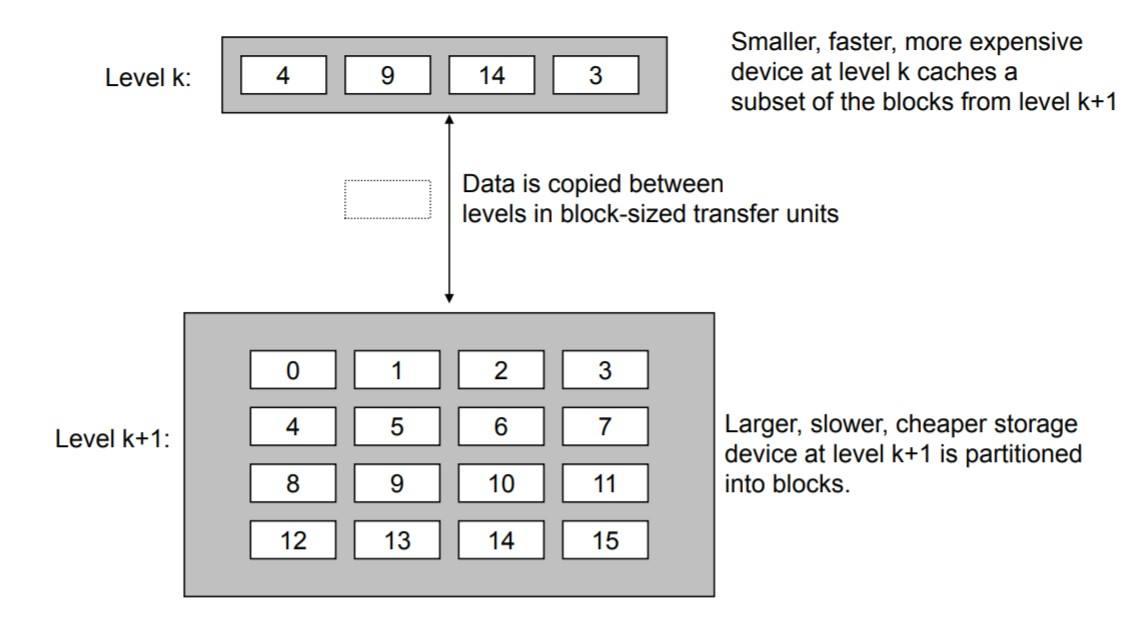
\includegraphics[scale=0.5]{CachePrinziep.jpg}
				\end{center}
			\end{minipage}


		\begin{minipage}[t]{0.45\textwidth}
			\subsubsection{Cache Hit}
				\begin{itemize}
					\item Wenn Ein Programm Daten von einem Objekt $d$ braucht, wird geschaut, ob d in einem der Blöcke
						auf Level $k$ gespeichert ist
					\item Wenn $d$ in dem Cache auf Level $k$ gefunden wird, nennt man das einen \textbf{Chache Hit}
					\item Das Programm lie\ss t dann $d$ direkt aus dem Level $k$ 
					\item Da Level $k$ schneller ist als $k+1$ ergibt sich dadurch ein Geschwindigkeitsvorteil
					\item Bemerkung: auch wenn L1, L2 und L3 als Cache alle als SRAM ausgeführt sind, 
						gibt es trotzdem Geschwindigkeitsunterschiede
				\end{itemize}
				\vfill%
		\end{minipage}
		\begin{minipage}[t]{0.45\textwidth}
			\subsubsection{Cache Miss}
				\begin{itemize}
					\item Wenn ein Programm Daten von einem Objekt $d$ braucht, wird geschaut, ob $d$ in einem der
						Blöcke auf dem Level $k$ gespeichert ist
					\item Wenn $d$ in dem Cache auf Level $k$ \textbf{nicht} gefunden wird, nennt man das einen \textbf{Cache Miss}
					\item Bei einem Cache Miss holt der Cache auf dem Level $k$ den Block mit $d$ von dem Cache auf Level $k+1$
					\item Möglicherweise muss dann ein existierender Block (wenn Cache voll) überschrieben werden
					\item Das s.g. \textit{Ersetzen} kann unterschiedlich erfolge:
						\begin{itemize}
							\item Zufallsersetzung
							\item Least-recently used (LRU) Ersetzung
						\end{itemize}
					\item Bedeutung der Lokalität beachten
				\end{itemize}
		\end{minipage}


		\subsubsection{Speicherhierarchie}
			\begin{minipage}{0.5\textwidth}
				\begin{itemize}
					\item Caching in Modernen Rechnersystemen (siehe Abbildung)
					\item Die Blöcke werden grö\ss er 
					\item Die Verzögerung (Latenz) wird grö\ss er
				\end{itemize}
			\end{minipage}
			\begin{minipage}{0.45\textwidth}
				\begin{center}
					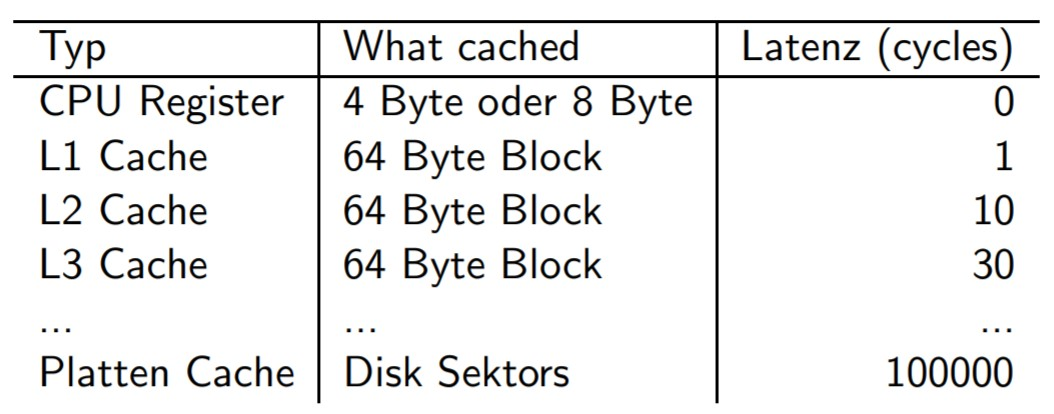
\includegraphics[scale=0.4]{CacheSpeicherhierarchie.jpg}
				\end{center}
			\end{minipage}


		\subsubsection{Cachehierarchie ARM/Intel Core i7}
			\begin{minipage}{0.5\textwidth}
				\begin{itemize}
					\item Von-Neumann und Harvard differenzierung nicht kommplett möglich
					\item L1 Cache Harvard, L2 Von-Neumann
				\end{itemize}

				\vspace{0.4cm}
				\begin{center}
					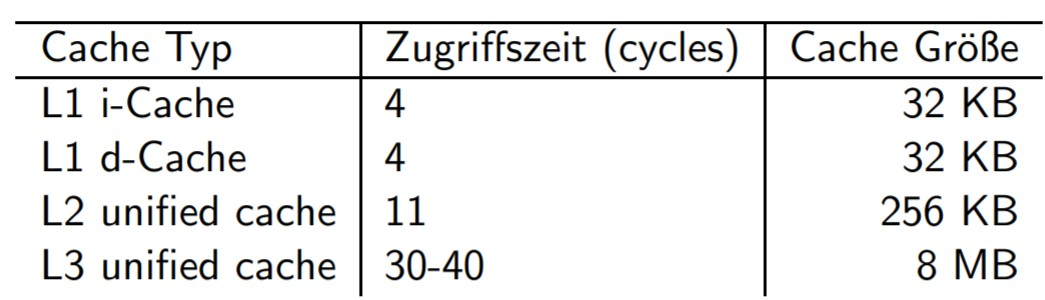
\includegraphics[scale=0.3]{CacheCharakteristischeWerte.jpg} \\
					Charakteristische Werte - Intel
				\end{center}
			\end{minipage}
			\begin{minipage}{0.45\textwidth}
				\begin{center}
					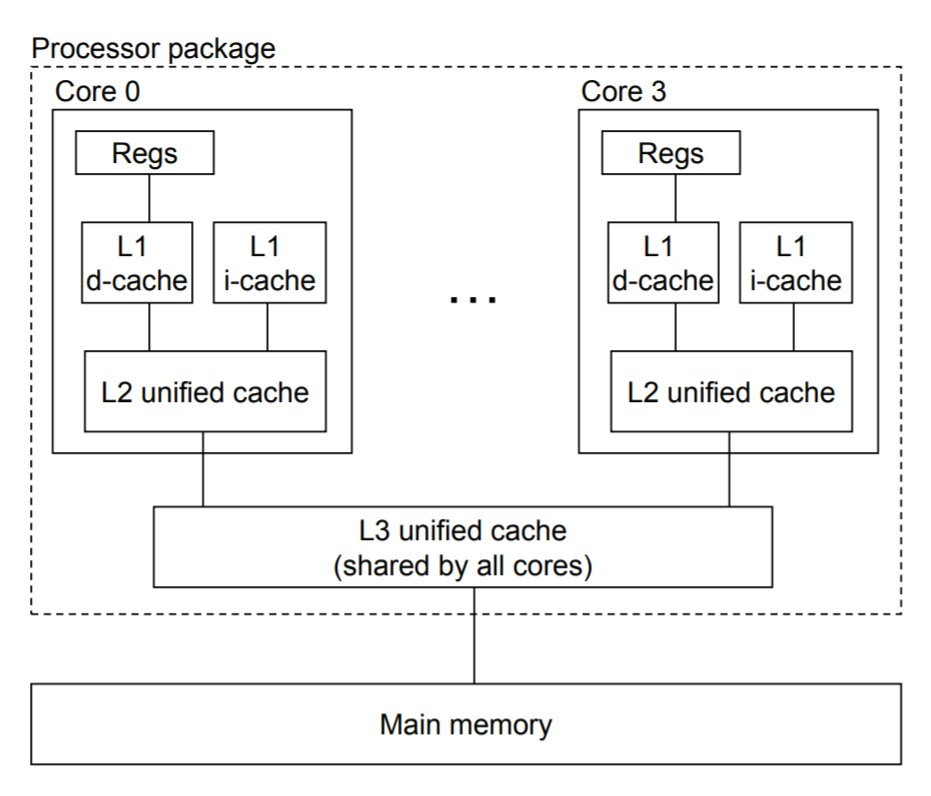
\includegraphics[scale=0.4]{Cachehierarchie.jpg}
				\end{center}
			\end{minipage}
			
			\vspace{1cm}
			\begin{minipage}[t]{0.5\textwidth}
				\subsubsection{ARM}
				\begin{itemize}
					\item Getrennte Caches für Daten (d-cache) und Instruktionen (i-cache) auf Level 1
					\item ARM Cortex - A53 MPCore Processor, Technical Reference Manual
				\end{itemize}
			\end{minipage}
			\begin{minipage}[t]{0.45\textwidth}
				\subsubsection{Intel Core i7}
				\begin{itemize}
					\item Getrennte Caches für Daten (d-cache) und Instruktionen (i-cache) auf Level 1
					\item Alle SRAM Cache Speicher sind auf dem CPU Chip (on die)
				\end{itemize}
			\end{minipage}


\newpage
\section{Maschinennahe Programmierung}
	\subsection{Phasen der Übersetzung}
		\paragraph{} Phasen der Übersetzung
		\begin{itemize}
			\item Das C Programm ist für den Menschen verständlich
			\item Zum Ausführen auf Rechnersystem muss es in Maschinenbefehle übersetzt werden
			\item Beispiel: gcc -o hello hello.c
		\end{itemize}

		\begin{center}
			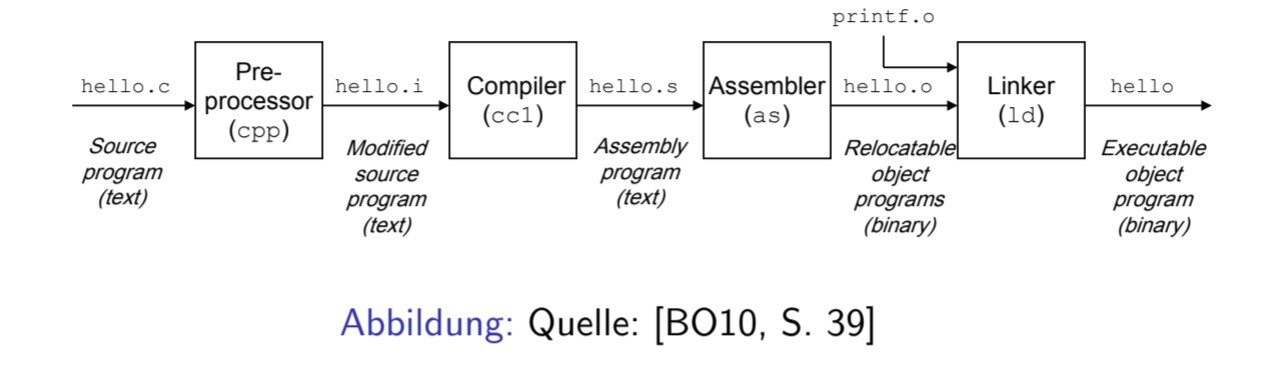
\includegraphics[scale=0.55]{PhasenDerUebersetzung.jpg}
		\end{center}

		\textbf{Phase Eins - Preprocessor}
		\begin{itemize}
			\item hello.c $\rightarrow$ hello.i
			\item Aufarbeiten von Direktiven (Befehle mit \# )
			\item Vorbereitung zur assemblierung
		\end{itemize}
		\vspace{0.5cm}

		\textbf{Phase Zwei - Compiler}
		\begin{itemize}
			\item hello.i $\rightarrow$ hello.s
			\item C-Programm in Assemblerprogramm
		\end{itemize}
		\vspace{0.5cm}

		\textbf{Phase Drei - Assembler}
		\begin{itemize}
			\item hello.s $\rightarrow$ hello.o (Maschinensprache)
			\item Ergebnis ist ein Objektprogramm
		\end{itemize}
		\vspace{0.5cm}

		\textbf{Pashe Vier - Linker/Binder}
		\begin{itemize}
			\item hello.o $\rightarrow$ hello (Ausführbares Programm)
			\item Zusammenfügen verschiedener Module
			\item Zum Beispiel externer Funktionen die Imprtiert werden (printf aus stdio.h)
		\end{itemize}
		\vspace{0.5cm}

		\paragraph{} Bei der Ausführung des Programms wird in der Shell der Befehl
		\texttt{./helo} ausgeführt. Die Shell ist ein Kommandozeileninterpreter der dann
		das Programm helo auf der Festplatte ausführt.



	\subsection{Ausführung eines Programmes}
		\paragraph{} Wir betrachten die Ausführung eines Programmes, als Beispiel \texttt{hello}
		mittels der Shell an einer Beispielhaftendarstellung eines Rechnersystems.

		\begin{center}
			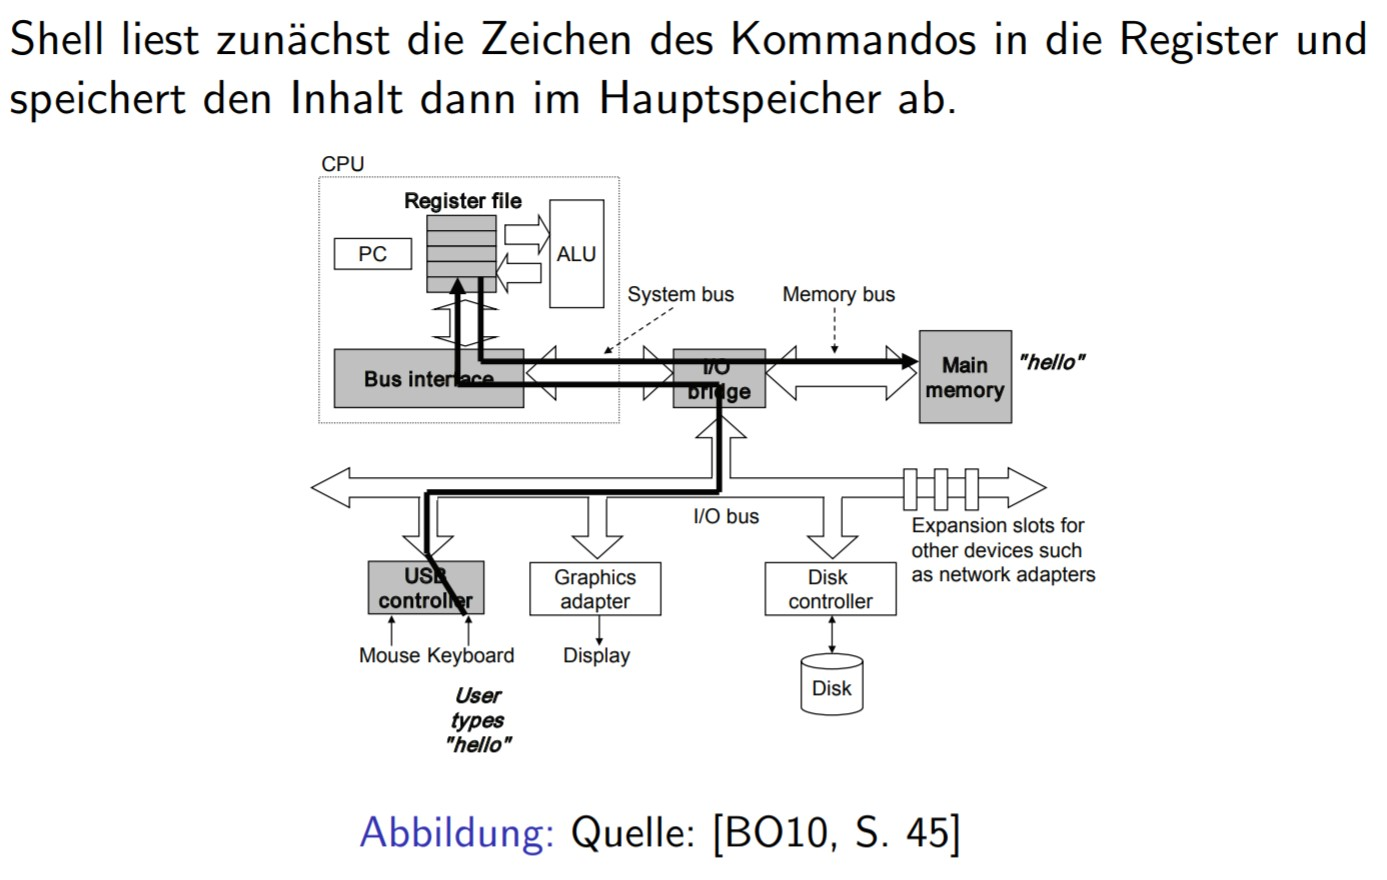
\includegraphics[scale=0.5]{AusfuehrungVonHello01.jpg} \\
			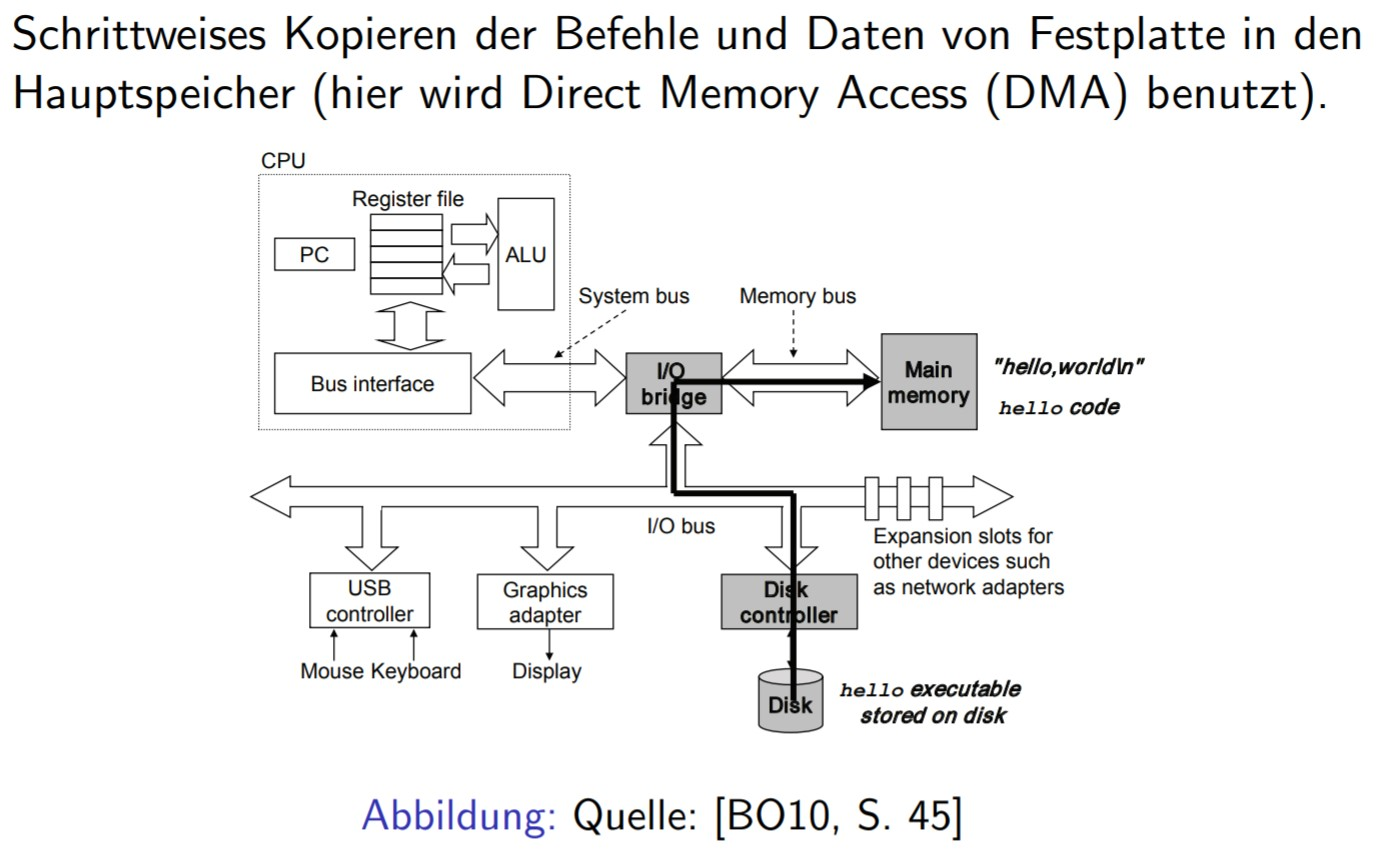
\includegraphics[scale=0.5]{AusfuehrungVonHello02.jpg} \\
			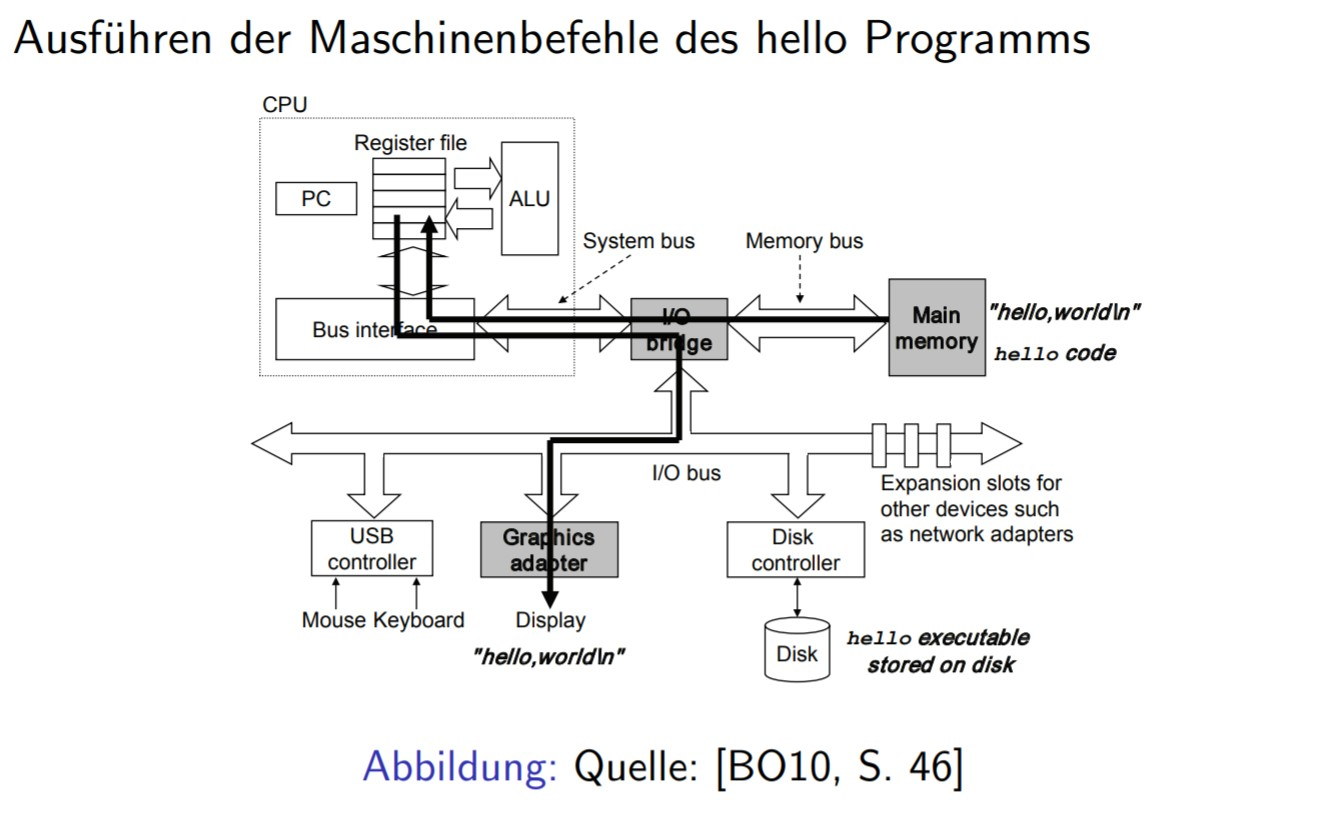
\includegraphics[scale=0.5]{AusfuehrungVonHello03.jpg}
		\end{center}


	\subsection{Compilieren, Assemblieren und Linken}
		\paragraph{Compilieren} Diskussion der Assemblerprogramme
		\begin{itemize}
			\item Die Übersetzung in den verschieden Phasen ist nicht eindeutig,
				ein Programm kann zu mehreren Übersetzungen führen
			\item Nicht alle Elemente werden in Assembler abgebildet, manche, z.B. triviale,
				Dinge können "weggelassen" werden
			\item Beispiel:
				\begin{itemize}
					\item Nicht jede lokale Variable wird gespeichert, manche werden nur in Register realisiert
					\item Manches wird direkt bei der Übersetzung berechnet
					\item \dots
				\end{itemize}
		\end{itemize}

		\paragraph{Assemblieren} ist der Prozess des Übersetzens von Assemblerprogrammen 
		(Mnemonics) in Maschinensprache: \\
		Ein Assembler ist ein Programm, das die Aufgabe hat, Assemblerbefehel in Maschinecode
		zu transformieren und dabei:
		\begin{itemize}
			\item SymbolischeNamen (z.B. Labels bei Rücksprungmarken) Maschinenadressen zu zuweisen
			\item und eine oder mehrere Objektdatei(en) zu erzeugen.
			\item \textbf{Crossassembler:} Assembler läuft aus System X, generiert Maschinencode für Plattform Y
			\item \textbf{Disassembler:} Übersetzung von Maschinensprache ind Assemblersprache,
				üblicherweise Verlust von Kommentaren und symbolischen Name \\
		\end{itemize}

		\noindent Arbeitsweise und Probleme:
		\begin{itemize}
			\item 1. Schritt:
					\begin{itemize}
						\item Auffinden von Speicherpositionen mit Marken. Beziehungen zwischen
							symbolischen Namen und Adressen werden bekannt
						\item Übersetzung des Assemblerprogrammbefehls in legale Instrkution
							(mittels Opcodes etc.)
					\end{itemize}
			\item Probleme beim 1. Schritt, Beispiel: \\
					Das Programm wird Zeile für Zeile abgearbeitet, bei Vorwärtsprüngen kann der Zielmarker
					also noch unbekannt sein. Daher wird das Programm zwei mal durchlaufen, beim ersten mal 
					werden alle Maschinenadressen zugeordnet, beim zweiten mal wird der Code erzeugt.
			\item 2. Schritt: Objektdateien werden erzeugt. Enthält Maschinencode, Daten und Verwaltungsinformation \\
					Ist im allgemeinen nicht ausführbar, da sie auf andere Dateien verweist (nächster Schritt: Linker)
			\item Probleme beim 2. Schritt: \\
				1. Fall:
					\begin{itemize}
						\item Assembler verwendet absolute Adressen
						\item Laden ist unmittelbar möglich, aber:
						\item Verschieben des Programms im Speicher ist nicht möglich
					\end{itemize}
				2. Fall:
					\begin{itemize}
						\item Assembler verwendet relative Adressen
						\item Es werden mehr, oder genau eine Objektdatie erzeugt, aber:
						\item weitere Transformationsschirtte sind notwendig $\Rightarrow$ Linker
					\end{itemize}
		\end{itemize}

		

		\paragraph{Linker/Binder}
		\begin{itemize}
			\item \textbf{Definiton Linker} \\
				Der Linker verbindet oder linked verschieden Objektfiles und macht aus ihnen
				ausführbare Objektprogramme indem noch offene Referenzen aufgelöst werden
			\item Das Objektprogramm kann durhc einen Lader ausgeführt werden
			\item \textbf{Definition Lader} \\
				Ein loader (Lader) Ist ein Systemprogramm, das Objektprogramme in den
				Speicher lädt und ggf. ihre Ausführung initialisiert
			\item Dazu wird das Objektprogramm in den Speicher kopiert \\
		\end{itemize}

		\noindent Arbeitsweise eines Laders:
		\begin{itemize}
			\item Ein Programmmodul (Lademodul) wird beginnend mit bei einer Startadresse
				in den Hauptschpeicher geladen
			\item Varianten:
					\begin{itemize}
						\item absolutes laden (absolute loading)
						\item relatives laden (relocatable loading)
						\item dynamisches laden zur Laufzeit (dynamic run time loading)
					\end{itemize}
		\end{itemize}


	

	\subsection{Kontrolloperationen - Statusbits}
		\paragraph{Carry und Overflow} \mbox{} \\
		Statusflags (die wichtigsten):
		\begin{itemize}
			\item C - Carryflag (Übertragsflag)
			\item Z - Zeroflag (Nullflag)
			\item N - Negativflag (Vorzeichenflag)
			\item V - Overflowflag (Überlaufflag)
		\end{itemize}
		Verwendungszweck:
		\begin{itemize}
			\item Z: Hochsprache $\rightarrow$ t == 0
			\item N: Hochsprache $\rightarrow$ t < 0
		\end{itemize}
		\vspace{0.5cm}

		\paragraph{} Ein Carrybit tritt auf, wenn bei einer Rechnung
		Bits überlaufen, also über die Wortlänge heraus, die Rechnung aber 
		korrekt ist. Z.B.: \\ 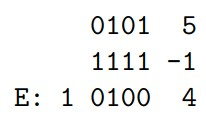
\includegraphics[scale=0.4]{ExsampleCarrybit.jpg} \\

		Ein Overflowbit tritt auf, wenn bei Berechnung durch Übertrag ein falsches
		Ergebnis entsteht: 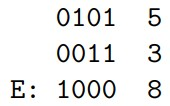
\includegraphics[scale=0.4]{ExsampleOverflow.jpg} \\

		Ein Negetivflag tritt auf, wenn die Zahl negativ ist, also in 2K Darstellung
		das höchstwertige bit 1 ist.



\newpage
\section{Konzepte der maschinennahen Programmierung}
	\subsection{Allgemeins}
		\paragraph{} Operanden (immediates) können bei manchen Befhelen verwendet werden. \\
		Sie werden durch ein \# vorangegangen. Ein Direktwert ist eine 12-Bit breite 
		Zahl im Zweierkomplement.
		\paragraph{} Maschinenbefehle (Mnemonics)

	\subsection{Lesen und Schreiben}
		Befehle:
		\begin{itemize}
			\item mov: Move  (r, r/\# )
			\item ldr: Load  (r, [Adresse] ) - Adresse: r, \#
			\item str: Store (r, [Adresse] ) - Adresse: r, \#
			\item Können auch auf bytes arbeiten: ldrb, strb
		\end{itemize}
		\vspace{0.5cm}

		Befehle:
		\begin{itemize}
			\item mov r5, \# 0
			\item ldr r7, [r5, + 0xC]
		\end{itemize}
		\vspace{0.5cm}
			Adressarithmetik:
		\begin{itemize}
			\item Basisadresse (r5) plus Distanz (offset) (0xC)
			\item Nach Abarbeitung r7 == 0x40F30788
		\end{itemize}
		\begin{center}
			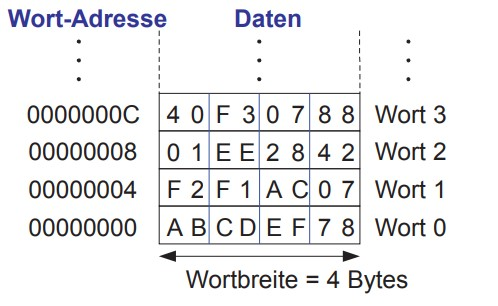
\includegraphics[scale=0.55]{LoadBeispiel.jpg}
		\end{center}
		\vspace{0.5cm}

		Das Schreiben funnktioniert auf analoge weise.



	\subsection{Nutzen des Hauptspeichers}
		\begin{itemize}
			\item Bisher wurden Daten direkt in Register geschrieben (z.B. mov)
			\item Man kann Werte auch direkt durch angabe der Variablennamen laden
			\item Vorraussetzung: \\
				\textcolor{white}{.} \hspace{0.5cm} \texttt{.data /* Daten Bereich */} \\
				\textcolor{white}{.} \hspace{0.5cm} \texttt{var1: .word 5 /* Var1 im Speicher, Wert 5 */} \\
				\textcolor{white}{.} \hspace{0.5cm} \texttt{... main: ...} \\
				\textcolor{white}{.} \hspace{0.5cm} \texttt{adr\_var1: .word var1 /* Adresse von Var1 */}
			\item Dies geht direkt: \\ 
				\textcolor{white}{.} \hspace{0.5cm} \texttt{ldr r0, var1}
			\item Oder indirekt über die Adressen:\\ 
					\textcolor{white}{.} \hspace{0.5cm} \texttt{ldr r0, adr\_var1 /* laedt Adresse von var1 in r0 */} \\ \vspace{0.15cm}
					\textcolor{white}{.} \hspace{0.5cm} \texttt{ldr r1, [r0] /* Lade inhalt von Adresse r0 in r1 */} \\
				Eine vereinfachte Syntax stellt dabei \texttt{=var1} dar: \\
					\textcolor{white}{.} \hspace{0.5cm} \texttt{ldr r0, =var1 /* laedt Adresse von var1 in r0 */} \\
					\textcolor{white}{.} \hspace{0.5cm} \texttt{ldr r1, [r0] /* Lade inhalt von Adresse r0 in r1 */} \\
		\end{itemize}
		\begin{center}
			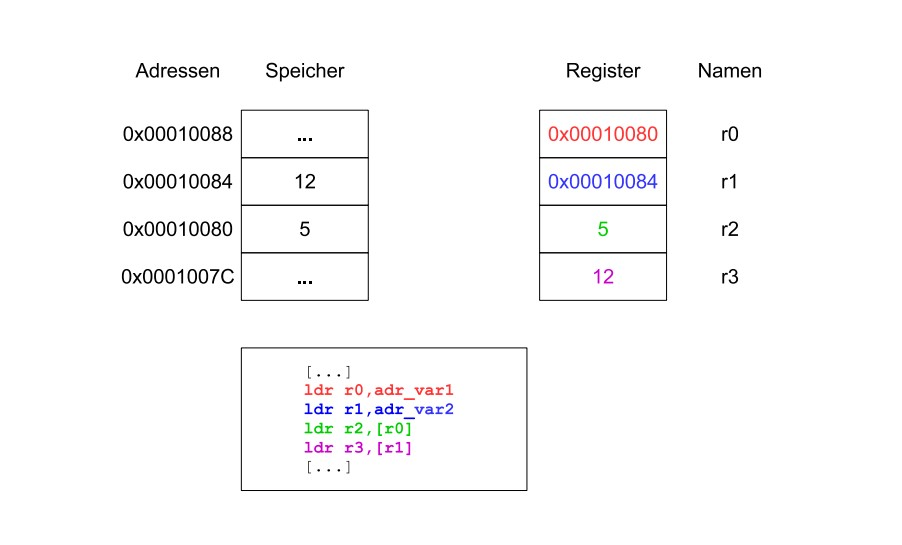
\includegraphics[scale=0.45]{RegisterUndHauptspeicher.jpg}
		\end{center}


	\subsection{Sprünge / Verzweigungen}
		Befehle:
		\begin{itemize}
			\item b target: branch target - springe zu target
			\item beq target: branch equals - bedingter Spring
			\item cmp: Compare - vergleicht zwei register, für beq oder bne
		\end{itemize}

		\paragraph{} Bei Sprüngen wird immer zu einem target/label gesprungen. Dies sind
		Namen für Stellen (Adressen) im Programm. Sie müssen anders als Mnemonics hei\ss en
		Labels müssen mit Doppelpunkt abgeschlossen werden. \\
		Optional kann durch einen Vergleich (cmp) ein Bedingter Sprung ausgeführt werden. 
		Dabei setzt cmp die zu vergleichenden Register fest, und der branch befehl handelt
		abhängig von dem Vergleich. \\
		Bei äquivalenten ausdrücken in Hochsprachen wird meist das gegenteil abgefragt.
		\begin{center}
			Unbedingt \hspace{8cm} Bedingt \hspace{2cm} \textcolor{white}{.} \\
			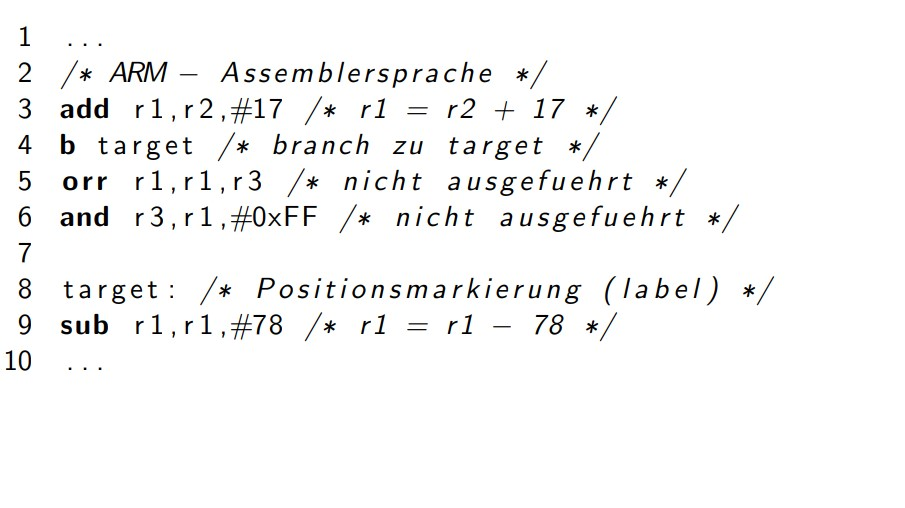
\includegraphics[scale=0.35]{UnbedingteSpruenge01.jpg}
			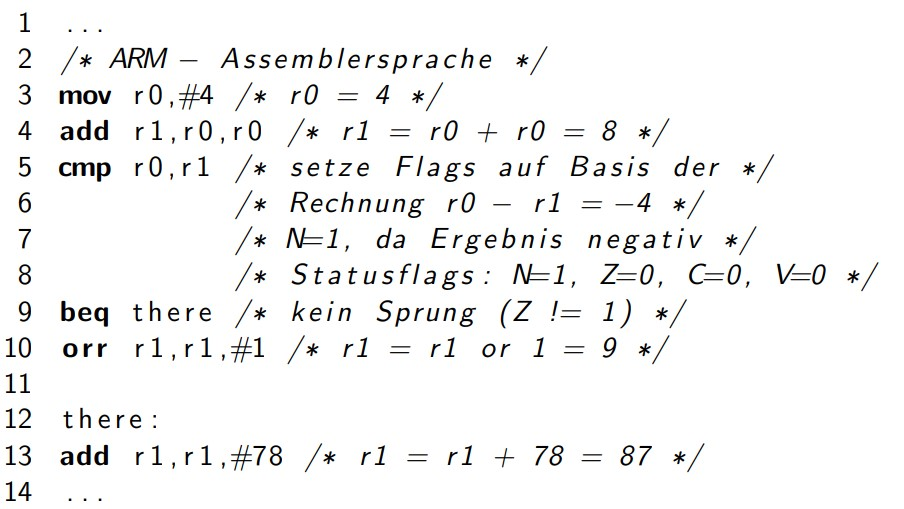
\includegraphics[scale=0.35]{BedingteSpruenge01.jpg}
		\end{center}

		\paragraph{} Beispiele für Anweisungen:
		\begin{center}
			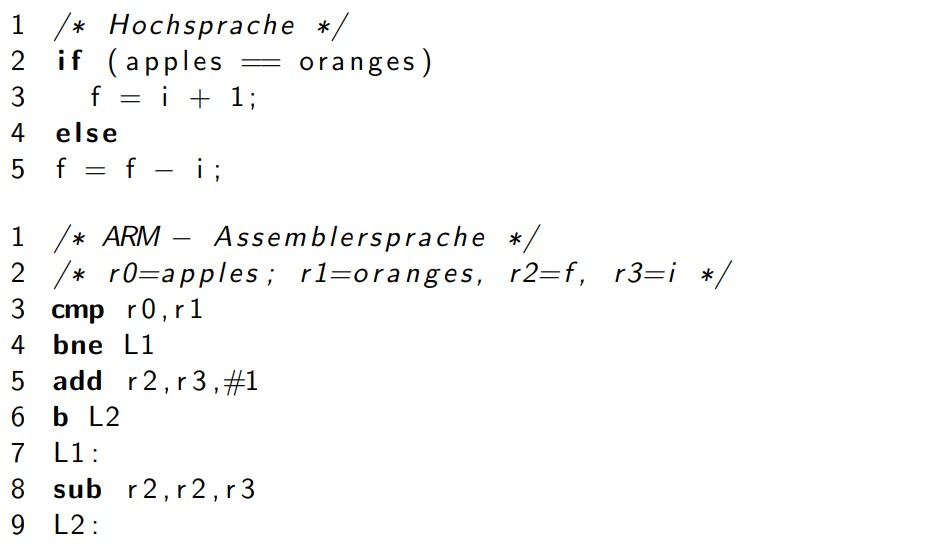
\includegraphics[scale=0.35]{BedingteSpruengeIf01.jpg}
			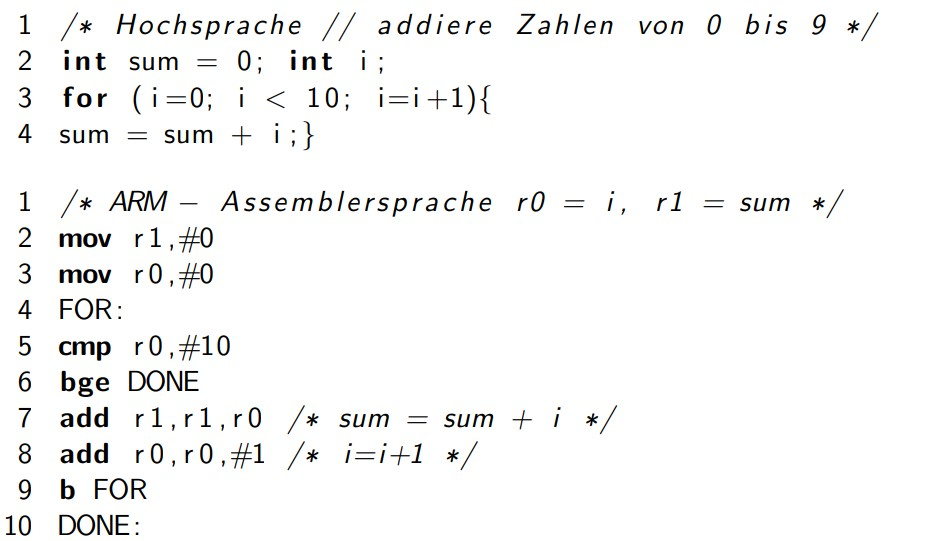
\includegraphics[scale=0.35]{BedingteSpruengeFor01.jpg}
		\end{center}



	\subsection{Datenfelder (Arrays)}
		\paragraph{} Prinziep: \\
		Ein Array besteht aus mehreren Worten, dies ist nützlich um aus eine große
		Zahl von Daten gleichen Typs zuzugreifen \\
		Auf die Elemente wird über einen Index zugegriffen. Konkret bedeutet das, dass
		auf die Basisadresse immer ein Offset addiert wird, genau eine Wortlänge, um 
		zum nächsten Element zu kommen:
		\begin{center}
			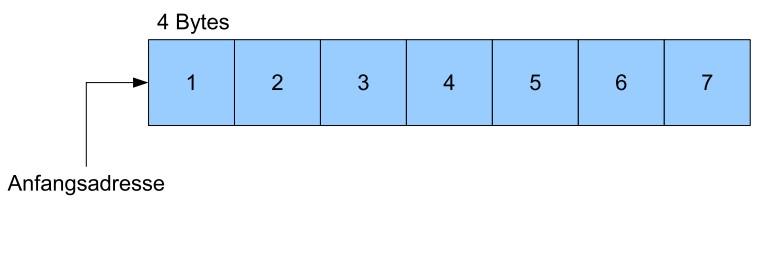
\includegraphics[scale=0.5]{ArrayDarstellung01.jpg}
			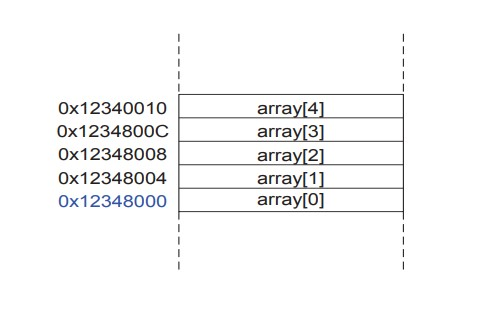
\includegraphics[scale=0.5]{ArrayDarstellung02.jpg}
		\end{center}
		
		\paragraph{} Zugriff: \\
		Der Zugriff auf das Array verläuft mittels Adressarithmetik. Dabei wird auf 
		die Basisadresse immer das i-vielfache eines Offsets addiert: \\
		\texttt{1} \hspace{0.2cm} \texttt{mov r0, \#0x1400000000 /* Basisadresse in r0 */} \\
		\texttt{2} \hspace{0.2cm} \texttt{mov r1, \#0 /* r1 = 0, Laufvariable i */} \\
		\texttt{3} \hspace{0.2cm} \texttt{lsl r2, r1, \#2 /* r2 = i * 4, leftishit logic */} \\
		\texttt{4} \hspace{0.2cm} \texttt{ldr r3, [r0, r2] /* r3 = array[i] */} \\
		
			
			
			
	\subsection{Unterprogramme}
		\paragraph{Einführung}
		\begin{itemize}
			\item Helfen bei strukturierter Programmierung
			\item Aus einem Programm (Hauptprogramm) wird eine Teilprogramm ausgeführt
			\item Makrotechnik vs Unterprogrammtechnik
		\end{itemize}
		Zu beachten ist:
		\begin{itemize}
			\item Wie erfolgt die Parameterübergabe und wie werden Ergbenisse ausgetauscht
			\item Sichtabrkeit von Varibalen, global vs lokal
			\item Jede Variable besitzt während ihrer Lebensdauer einen Speicherplatz
		\end{itemize}
		\vspace{0.2cm}
		
		\noindent Regeln:
		\begin{itemize}
			\item Aufrufer:
				\begin{itemize}
					\item Übergibt Argumente (aktuelle Parameter) and Aufgerufenen
					\item Springt Aufgerufenen an
				\end{itemize}
			\item Aufgerufener:
				\begin{itemize}
					\item Führt Funktion / Prozedur aus
					\item Gibt Ergebnis (Rückgabewert) and Aufrufer zurück (für Funktion)
					\item \textbf{Wichtig:} Darf keine Register oder Speicherstellen überschreiben die im Aufrufer genutzt werden \\
							$\Longrightarrow$ Stacks als Lösung
				\end{itemize}
		\end{itemize}
		\vspace{0.4cm}


		\paragraph{Makro- vs Unterprogrammtechnik}

		\paragraph{} Makrotechnik: \\
		\begin{minipage}{0.6\textwidth}
			\begin{figure}[H]
					\begin{itemize}
						\item Das Teilprogramm wird an benötigten Stellen einkopiert
						\item Dazu wird dem TP ein, dem s.g. Makro, ein Name zugeordnet (Makroname)
						\item Das passiert durch die s.g. Makrodefiniton
						\item An den zu einkopierenden Stellen wird dann der Makroname genannt
						\item $\Rightarrow$ Makroaufruf
					\end{itemize}
				\end{figure}
			\end{minipage} \hfill
		\begin{minipage}{0.35\textwidth}
			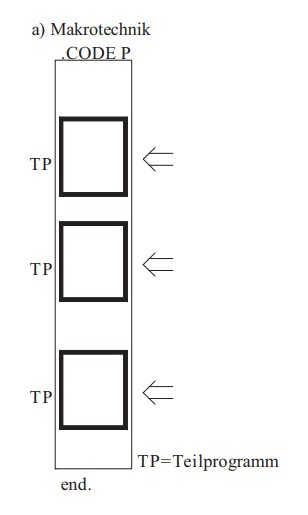
\includegraphics[scale=0.4]{Makrotechnik01.jpg}
		\end{minipage}

		\paragraph{} Unterprogrammtechnik: \\
		\begin{minipage}{0.6\textwidth}
			\begin{figure}[H]
				\begin{itemize}
					\item Hier ist das Unterprogramm nur einmal im Code vorhanden
					\item And den Stellen an denen das Unterprogramm ausgeführt werden soll \\
							erfolgt der Aufruf durch einen Sprungbefehl
					\item Am Ende erfolgt die Rückkehr in das aufrufende Programm
					\item Rückkehradresse wird gespeichert
				\end{itemize}
			\end{figure}
		\end{minipage}
		\begin{minipage}{0.35\textwidth}
			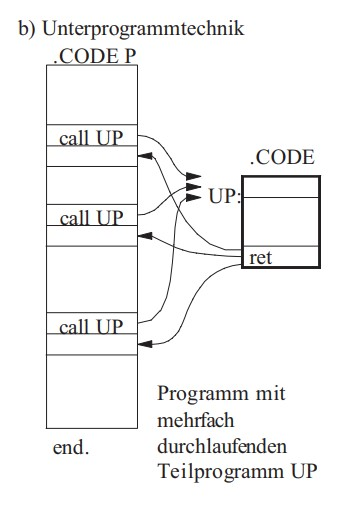
\includegraphics[scale=0.4]{Unterprogrammtechnik01.jpg}
		\end{minipage}

		\paragraph{Beispiel in Assembler}
		\begin{center}
			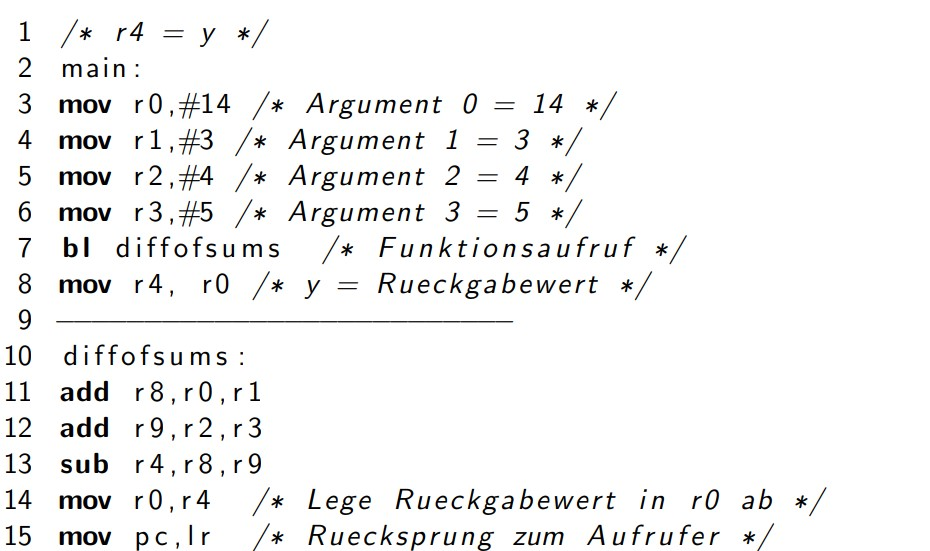
\includegraphics[scale=0.35]{UnterprogrammBeispiel.jpg}
			\includegraphics[scale=0.35]{UnterprogrammBeispielErklärung.jpg}
		\end{center}
			

	\subsection{Stacks}
		\paragraph{Einleitung}
		\begin{itemize}
			\item Stacks (Stapel- Kellerspeicher) sind Speicher zur temporären Nutzung
			\item Bekannt aus AuD - last in first out LIFO
			\item Dynamische Speicher zuweisung
			\item Wächst bei ARM nach unten (von hohen zu niedrigen Speicheradressen)
			\item Stapelzeiger ("stack pointer"): sp (r13)
			\item zeigt auf zuletzt auf dem Stapel abgelgtes Datenelement
		\end{itemize}

		\paragraph{Implementierung in Teilprogramme}
		\begin{itemize}
			\item TPs dürfen keine Seiteneffekte haben
			\item Problem: doffossums überschreibt die drei Register r8, r9, r4
		\end{itemize}
		\begin{minipage}{0.5\textwidth}
			\includegraphics[scale=0.35]{DiffOfSumsNormal.jpg} \\ 
			\includegraphics[scale=0.3]{StackBehaviour.jpg}
		\end{minipage}
		\begin{minipage}{0.45\textwidth}
			\includegraphics[scale=0.35]{DiffOfSumsWithStack.jpg}
		\end{minipage}
		\vspace{0.2cm}

		Vor Aufruf des Unterprogramms muss die Rücksprungadresse gespeichert werden, z.B.:
		\begin{itemize}
			\item Mittels mov: \\
					\textcolor{white}{.} \hspace{0.2cm} \texttt{mov r10, lr /* sichern der Rücksprungadresse in r10 */} \\
					\textcolor{white}{.} \hspace{0.2cm} \texttt{bl diffofsums /* Funktionsaufruf */} \\
					\textcolor{white}{.} \hspace{0.2cm} \texttt{mov r4, r0 /* y = Rückgabewert */} \\
					\textcolor{white}{.} \hspace{0.2cm} \texttt{mov lr, r10 /* herstellen der Rücksprungadresse */}
			\item Mittels pop und push als Pseudointrsuktionen: \\
					\textcolor{white}{.} \hspace{0.2cm} \texttt{push \{lr\} /* sichern der Rücksprungadresse in r10 */} \\
					\textcolor{white}{.} \hspace{0.2cm} \texttt{bl diffofsums /* Funktionsaufruf */} \\
					\textcolor{white}{.} \hspace{0.2cm} \texttt{mov r4, r0 /* y = Rückgabewert */} \\
					\textcolor{white}{.} \hspace{0.2cm} \texttt{pop \{lr\} /* herstellen der Rücksprungadresse */}
		\end{itemize}



	\subsection{Rekursion}
		\paragraph{Prinziep} \mbox{} \\
		\begin{minipage}{0.6\textwidth}
			Das Prinziep hinter der Rekursion, ist das wiederholte aufrufen von Funktionen
			in sich selber. Konkret Wird die Funktion im Hauptptrogramm aufgerufen und ruft sich
			unter bestimmten Bedingungen selsbt wieder auf. Tritt der Fall ein, dass sie sich nicht
			selsbt aufruft, wird das ergebnis an die Aufrufende Fukntion zuruückgeben. Diese kann
			ihr Ergebnis wiederum zuruückgeben usw.

			\begin{itemize}
				\item Die Abbildung der Inkarnation zeig, dass es zwie verschiedene Rücksprungadressen gibt
				\item RA\_1 = Adresse im Hauptprogramm
				\item RA\_2 = Adresse im Unterprogramm (für alle Rekursionstufen gleich)
			\end{itemize}
		\end{minipage}
		\begin{minipage}{0.35\textwidth}
			\includegraphics[scale=0.5]{RekursionVisualisierung.jpg}
		\end{minipage}
		\vspace{0.8cm}

		\noindent Beispielprogramm mit Rekursion: \\
		%\vspace{0.4cm}
		\begin{minipage}{0.7\textwidth}
			\textcolor{white}{.} \hspace{0.4cm} \texttt{push \{lr\}} \\
			\textcolor{white}{.} \hspace{0.4cm} \texttt{mov r0, \#3 /* Fak von 3 */} \\
			\textcolor{white}{.} \hspace{0.4cm} \texttt{bl fak} \\
			\textcolor{white}{.} \hspace{0.4cm} \texttt{mov r1, r0 /* Ergenis von fak in r1} \\
			\textcolor{white}{.} \hspace{0.4cm} \texttt{...} \\ \mbox{} \\

			\textcolor{white}{.} \hspace{0.4cm} \texttt{fak:} \\
			\textcolor{white}{.} \hspace{0.4cm} \texttt{sub sp, sp, \#8 /* Speicher Stack reservieren */} \\
			\textcolor{white}{.} \hspace{0.4cm} \texttt{str r0, [sp, \#4] /* sichern von r0 auf stack (3) */} \\
			\textcolor{white}{.} \hspace{0.4cm} \texttt{str lr, [sp] /* sichern Rücksprungadresse */} \\
			\textcolor{white}{.} \hspace{0.4cm} \texttt{cmp r0, \#1 /* Rekursionsende prüfen */} \\
			\textcolor{white}{.} \hspace{0.4cm} \texttt{blt else} \\
			\textcolor{white}{.} \hspace{0.4cm} \texttt{sub r0, r0, \#1 /* n = n - 1 */} \\
			\textcolor{white}{.} \hspace{0.4cm} \texttt{bl fak /* Funktionsaufruf */} \\
			\textcolor{white}{.} \hspace{0.4cm} \texttt{ldr r1, [sp, \#4] /* laden von n */} \\
			\textcolor{white}{.} \hspace{0.4cm} \texttt{mul r0, r1, r0 /* fak (n-1)*n */} \\
			\textcolor{white}{.} \hspace{0.4cm} \texttt{fin:} \\
			\textcolor{white}{.} \hspace{0.4cm} \texttt{ldr lr, [sp] /* laden Rückkehradresse} \\
			\textcolor{white}{.} \hspace{0.4cm} \texttt{add sp, sp, \#8 /* Speicher Stack freigeben */} \\
			\textcolor{white}{.} \hspace{0.4cm} \texttt{bx lr /* Sprung zum Aufrufer */} \\
			\textcolor{white}{.} \hspace{0.4cm} \texttt{else:} \\
			\textcolor{white}{.} \hspace{0.4cm} \texttt{mov r0, \#1 /* Rekursionsanker */} \\
			\textcolor{white}{.} \hspace{0.4cm} \texttt{b fin} \\
		\end{minipage}
		\begin{minipage}{0.25\textwidth}
			\includegraphics[scale=0.35]{FaklutaetC.jpg} \\
			\includegraphics[scale=0.5]{FakultaetStackBehaviour.jpg}
		\end{minipage}


		
	\subsection{Zusammenfassung Unterprogrammaufrufe}
		\begin{itemize}
			\item Aufrufer
				\begin{itemize}
					\item Lege Aufrufparameter in Register oder Stack ab
					\item Sichere notwendige Registe auf Stack (z.B. lr)
					\item bl Aufgerufener
					\item Stelle gesicherte Register wieder her
					\item Hole evtl. Rückgabewert aus r0 (bei Funktionen)
				\end{itemize}
			\item Aufgerufener
				\begin{itemize}
					\item Sichere zu erhaltende verwendete Register auf Stack
					\item Führe Berechnung des Unterprograms aus
					\item Lege Rückgabewert in r0
					\item Stelle gesicherte Register wieder her
					\item Rücksprung zum Aufrufer: mov pc, lr
				\end{itemize}
			\item Unter Aufrufkonvention versteht man die Methode, mit der einem Unterprogramm Daten übergeben werden
		\end{itemize}


			
\newpage
\section{Gleitkommazahlen}
	\subsection{Zahlendarstellung - Visualisierung}
		\begin{minipage}{0.55\textwidth}
			\subsubsection{Darstellung Reeller Zahlen}
			\begin{itemize}
				\item Zwei Arten für reelle Zahlen
						\begin{itemize}
							\item Festkommadarstellung
							\item Gleitkommazahlen
						\end{itemize}
				\item Zur Festkommadarstellung
						\begin{itemize}
							\item Man lässt bei der internen Darstellung das Komma weg und
								merkt sich wo es stehen müsste
							\item Zum Programmbeginn wird die Kommastelle der entsprechenden Variable definiert
								und bleibt dann während des Programmablaufs fest
						\end{itemize}
			\end{itemize}
		\end{minipage}
		\begin{minipage}{0.4\textwidth}
			\begin{center}
				\includegraphics[scale=0.5]{Zahlendartsellung.jpg}
			\end{center}
		\end{minipage}


	\subsection{Gleitkommazahlen nach ANSI/IEEE 754}
			\begin{itemize}
				\item Bei Gleitkommadarstellung (halbarithmetisch Darstellung) ist die Kommastelle 
					Bestand der Zahl und kann sich im Laufe der Rechnung verändern
				\item Durch standartisierte Schreibweise/Darstellung braucht man Komma nicht 
					explizit angeben
				\item Floatingpoint Darstellung ist standartisiert nach ANSI/IEEE 754
				\item Hat sich weltweit durchgesetzt und dient als Grundlage
				\item 1985 verabschiedet, 2008 gab es eine Revision 
			\end{itemize}

			\vspace{0.3cm}
			\begin{center}
				Präziisionsformate: \\
				\includegraphics[scale=0.5]{Preaezisionsformate.jpg}
			\end{center}


			\vspace{0.5cm}
			\begin{itemize}
				\item Besonderheiten: Die Null kann (durch Normalisierung) nicht dargestellt werden
				\item Unendliche Zahlen, oder keine Zahlen, sollen auch dargestellt werden
			\end{itemize}
			\centerline{\includegraphics[scale=0.7]{GleitkommazahlenNullNaN.jpg}}


		\subsubsection{Beispiel Gleitkommazahl}
			\paragraph{} Eine Gleitkommazahl z wird als $z = \pm m * b^{\pm e}$ dargestellt, wobei m die Mantisse,
			e der Exponent und b die Basis des Exponenten ist. \\
			Zur Darstellung einer Gleitkommazahl wird folgendes benötigt: 
			\begin{itemize}
				\item Vorzeichen der Mantisse
				\item Betrag der Mantisse mit Komma
				\item Basis (ganze Zahl)
				\item Vorzeichen des Exponenten
				\item Betrag des Exponenten (ganze Zahl)
			\end{itemize}
			Um dies zu vereinfachen gibt es den ANSI/IEEE Standard:
			\begin{itemize}
				\item 1. Schritt - Zahl wird normalisiert: \\
					$654,321 \rightarrow 6,54321 * 10^2$ \\
					$0,006543 \rightarrow 6,543 * 10^{-2}$ \\
					$1001,011 \rightarrow 1,001011 * 2^3§ \\
					§0,011011 \rightarrow 1,1011 * 10^{-2}$ \\
					Definition: Eine gleitkommazahl heißt normalisiert, falls $b > |m| \geq 1$
				\item 2. Schritt - Charakteristik \\
					Die Charakterisitik, oder auch biased Exponent, ergibt sich durch die Addierung
					des Exponenten und des bias: $Charakterisitik = biased Exponent = Exponent + bias$
				\item 3. Schritt - Zusammensetzen \\
					Nun kann man die Zahl mit allen gegebenen Informationen Zusammensetzen
			\end{itemize}
			\begin{minipage}{0.5\textwidth}
				\begin{center}
					\includegraphics[scale=0.45]{CharakteristikBeispiel.jpg}
				\end{center}
			\end{minipage}
			\begin{minipage}{0.45\textwidth}
				\begin{center}
					\includegraphics[scale=0.45]{GleitkommazahlenBeispiele.jpg}
				\end{center}
			\end{minipage}



	\subsection{Verarbeitung reeller Zahlen in ARM}
		\begin{itemize}
			\item Bemerkung: \\
				Bzgl. der Nutzung von Gleitkommazahlen/Gleitkommaoperationen in Eingebetteten Systemen
				gibt es auch die Auffasung, dass man diese aufgrund von Geschwindigkeitsgründen vermeiden sollte.
				Ausnahme bildet das Vorhanden sein einer Hardware unterstützte Einheit für Gleitkommazahlen.
				Hat man keine Hardwre unterstützte Gleitkommaoperationen Einheit, kann man dies auch mit Integer
				Register simulieren.
		\end{itemize}

		\subsubsection{Code Analyse}
			\centerline{Addition zweier Gleitkommazahlen - float}
			\begin{minipage}{0.5\textwidth}
				\begin{center}
					\includegraphics[scale=0.6]{CCodeAdditionGleitkommazahlen.jpg}
				\end{center}
			\end{minipage}
			\begin{minipage}{0.45\textwidth}
				\begin{center}
					\includegraphics[scale=0.55]{AssemblerCodeAdditionGleitkommazahlen.jpg}
				\end{center}
			\end{minipage}

			\begin{itemize}
				\item Speicherung der Konstanten im Dezimalsystem (Binärzahl nach ANSI)
					\begin{itemize}
						\item $p = 5.4 -- 1085066445$
						\item $q = 12.6 -- 1095342490$
						\item 0100 0000 1010 1100 1100 1100 1100 1101
					\end{itemize}
				\item Neue Register und Befehle
					\begin{itemize}
						\item vldr.32 (load 32 bit?), vadd.32 (add 32 bit?),\dots
						\item s14 (single precision?), d7 (double precision?)
					\end{itemize}
			\end{itemize}


			\vspace{1.5cm}
			\centerline{Addition zweier Gleitkommazahlen - double}
			\begin{minipage}{0.5\textwidth}
				\begin{center}
					\includegraphics[scale=0.6]{CCodeAdditionGleitkommazahlenDouble.jpg}
				\end{center}
			\end{minipage}
			\begin{minipage}{0.45\textwidth}
				\begin{center}
					\includegraphics[scale=0.55]{AssemblerCodeAdditionGleitkommazahlenDouble.jpg}
				\end{center}
			\end{minipage}

			\begin{itemize}
				\item Speicherung der Konstanten im Dezimalsystem (Binärzahl nach ANSI) \\
					Beachte: Dabei werden zwei 32 Bit Register verwendet um ein 64 Bit Register darzustellen
					\begin{itemize}
						\item $p = 5.4 -- -1717986918 1075157401$
						\item $q = 12.6 -- 858993459 1076441907$
					\end{itemize}
				\item Neue Befehle und Register
					\begin{itemize}
						\item Ähnliche befehle wie bei float Berechnungen, angepasst auf double Werte
					\end{itemize}
			\end{itemize}


	\subsection{Studium der Datenblätter}
		\begin{minipage}{0.55\textwidth}
			\begin{itemize}
				\item Zwei Möglichkeiten Gleitkommazahlen zu verarbeiten:
					\begin{itemize}
						\item eine Funktionseinheit NEON
						\item eine Funktionseinheit VFP
					\end{itemize}
				\item Zusätzliche Register zur behandlung von Gleitkommazahlen
					\begin{itemize}
						\item s0 - s31 (Single Precision Register)
						\item d0 - d31 (Double Precision Register)
						\item q0 - q15 (128 Bit (2*Double) Precision Register)
					\end{itemize}
				\item Beide Funktionseinheiten benutzen die gleichen Register
			\end{itemize}
		\end{minipage}
		\begin{minipage}{0.4\textwidth}
			\centerline{\includegraphics[scale=0.5]{RegistersatzGleitkommazahlen.jpg}}
		\end{minipage}

		\centerline{\includegraphics[scale=0.6]{BefehleGleitkommazahlen.jpg}}


	\subsection{Gleitkommaeinheit}
		\begin{itemize}
			\item Die Berehcnung von Gleitkommazahlen wird seit langem in s.g. Gleitkomma-Coprozessoren  ausgelagert
			\item Gleitkomma-Coprozessoren besitzen häufig seperate Intruction-Pipelines z.B.
				\begin{itemize}
					\item Multiplikations und Additions (FMAC) Pipelines
					\item Divisions und Quadratwurzel (DS) Pipelines
				\end{itemize}
			\item Diese Pipelines können auch unabhängig voneinander operieren
		\end{itemize}

		\includegraphics[scale=0.5]{FMAC-Pipeline.jpg}
		\includegraphics[scale=0.5]{DS-Pipeline.jpg}



\newpage
\section{Mirkoarchitektur}
	\subsection{Terminologie}
		\begin{itemize}
			\item ISA - instruction set architecture (Menge der Verfügbaren Instrkutionen)
			\item RISC - recudes instruction set computer (kleine und schnell ausführbare ISA), z.B. ARM
			\item CISC - complex instruction set computer (schwergewichtige ISA), z.B. Intel
			\item SIMD - single instruction multiple data (vector processing), z.B. NEON
			\item VLIW - very long instruction word (static multi-issue), siperscalar processor
			\item $\mu$arch - microarchitecture (ISA Implementierung)
				\begin{itemize}
					\item instructions per cycle (IPC)
					\item instruction level parallelism (ILP) - RO07
					\item branch prediction (Sprungvorhersage)
				\end{itemize}
				\item Architekturzustand - dem Programmierer sichtbare Elemente
		\end{itemize}


	\vspace{0.8cm}
	\subsection{Allgemeines}
		Im allgeminen ist die Mirkoarchitektur eine Hardware Implementierung einer Architektur.
		Dabei wird zwischen Datenpfaden, die funktionale Blöcke verbinden, und Kontrollpfaden die Steursignale
		übermitteln, unterschieden.

		\subsubsection{Bearbeitung eines Befehls}
		Drei Phasen der Befehlsausführung:
		\begin{itemize}
			\item Aufgabe des Prozessors nzw. des Steuerstacks ist das lesen der 
				Befehle aus dem Speicher zu lesen - Befehlsholphase (instruction fetch)
			\item Nach dem holen des Befehls muss er dekodiert werden - Befehlsfekodierung (instruction decode)
			\item Nun wird der Befehl ausgeführt und der nächste geladen - Befehlsausführung (instruction execute)
		\end{itemize}


		\subsubsection{Takt und Taktfrequenz}
		\paragraph{} Die Prozesse eines Rechnersystems haben eine geminesame Zeitbasis 
		damit das Zzusammenspiel funnktioniert. Diese nennt man Takt. Die Taktfrequenz
		ergibt sich aus $f = \frac{1}{T}$ wobei $T$ die Periodendauer von einer steigenden
		Taktflanke zur nächsten angibt. $\Longrightarrow$ Je höher die Taktfrequenz, desto
		schneller wird verarbeitet.
		\begin{itemize}
			\item Bei CMOS Technologie steigt der Leistungsumsatz mit $P = U^2 * f * C_L$
		\end{itemize}

		\paragraph{} Implementierung: \\ \mbox{} \\
		\begin{minipage}{0.33\textwidth}
			\centerline{Eintakt-Implementierung}
			\begin{itemize}
				\item Jeder Befehl wird in einem Takt ausgeführt
			\end{itemize}
		\end{minipage}
		\begin{minipage}{0.33\textwidth}
			\centerline{Mehrtakt-Implementierung}
			\begin{itemize}
				\item Jeder Befehl wird in Teilschritte zerlegt
			\end{itemize}
		\end{minipage}
		\begin{minipage}{0.33\textwidth}
			\centerline{Pipelines-Implementierung}
			\begin{itemize}
				\item Jeder Befehl wird in parallel ausgeführte Teilschritte zerlegt
			\end{itemize}
		\end{minipage}


		\subsubsection{Rechnleistung eines Prozessors}
		Ausfürhung eines Programms:
		\begin{itemize}
			\item$ Ausführungszeit = (\#Instruktionen) * (\frac{Takte}{Instruktionen}) * (\frac{Sekunden}{Takte})$ \\
		\end{itemize}

		Definitonen:
		\begin{itemize}
			\item $\frac{Takte}{Instruktionen} = CPI$
			\item $\frac{Sekunden}{Takte} = Taktperiode$
			\item $\frac{1}{CPI} = \frac{Instruktionen}{Takt} = IPC$ 
		\end{itemize}

		\vspace{0.8cm}
	\subsection{Mikroarchitektur Prozessor}
		\subsubsection{Neumann / Harvard}
			Von-Neumann-Architektur
			\begin{itemize}
				\item gemeinsamer Speicher für Maschinenbefehle und Daten
			\end{itemize}

			Harvard-Architektur
			\begin{itemize}
				\item Befehlsspeicher und Datenspeicher sind getrennt
			\end{itemize}

			Speicher können asynchron gelesen werden, aber nur synchron geschrieben werden.


		\subsubsection{Elemente der Architektur/Prozessor (Eintakt)}
			\centerline{\includegraphics[scale=0.6]{BitfeldDarstellung.jpg}}
			\begin{itemize}
				\item Begin der Entwickling des Datenpfades mit dem Befehl \texttt{ldr}
				\item \texttt{ldr Rd, [Rn, imm12]} \\
					ldr = Befehl, Rd = Register destination, Rn = Register name, imm12 = 12Bit immediate
			\end{itemize}
			

			\begin{center}
				\includegraphics[scale=0.82]{ProzessorEinfach.jpg}
			\end{center}

			\begin{minipage}{0.45\textwidth}
				Register File:
				\begin{itemize}
					\item A1 .. A3 sind Registeradressen (4 Bits = 16 Register) \\
						RD1 (Register Data 1) Gelesene Daten aus A1
					\item A3 ist das Zielregister \\ 
						WD3 (Write Data 3) Geschriebene Daten in A3
					\item WE3 (Write Enable 3) steuert ob auf A3 geschrieben werden soll oder nicht \\
				\end{itemize}

				Instruction Memory:
				\begin{itemize}
					\item A
					\item RD
				\end{itemize}

			\end{minipage}
			\hspace{0.5cm}
			\begin{minipage}{0.45\textwidth}
				Status:
				\begin{itemize}
					\item Hier werden Statusflags zur verwendung in Operationen gespeichert \\
				\end{itemize}

				Programm Counter (PC):
				\begin{itemize}
					\item Unser wie bisher bekannte Programm Counter \\
				\end{itemize}

				Data Memory:
				\begin{itemize}
					\item 
				\end{itemize}
			\end{minipage}
			

	\vspace{0.8cm}
	\subsection{Eintakt-Prozessor}
		\subsubsection{Bitfelder und Prozessor Darstellung}
			\begin{center}
				\includegraphics[scale=0.45]{ProzessorLDR.jpg} \\
				\includegraphics[scale=0.45]{BitfeldLDR.jpg} \\
				\includegraphics[scale=0.45]{ProzessorBitfeldSTR.jpg} \\
				\includegraphics[scale=0.45]{ProzessorBitfeldADD.jpg} \\
				\includegraphics[scale=0.45]{ProzessorBranch.jpg} \\
				Branch-Befehle \\
				\includegraphics[scale=0.45]{ProzessorMitControllUnit.jpg} \\
				Prozessor mit Controll-Unit
			\end{center}
		
		
		\subsubsection{Phasen der Befehlsausführung: allgemein}
			Drei Phasen der Befehlsausführung:
			\begin{itemize}
				\item Befehlsholphase
				\item Befehlsdekodierung
				\item Befehlsasuführung
			\end{itemize}


		\subsubsection{Phasen der Befehlsausführung: ldr}
			% Am Besipiel von ldr Rd, [Rn, imm12]
			\begin{itemize}
				\item 1. Befehl holen \\
					Der \textbf{Programm Counter} lädt den Befehl aus dem \textbf{Instruction Memory}
				\item 2. Lesen der Quell-Operanden vom Registerfeld \\
					Rn Register aus dem \textbf{Bitfeld} des Befehls wird an A1 übergeben 
				\item 3. Erweitern des Offsets \\
					Eventueller Offset muss von seinen 12 Bit auf 32 Erweitert
					werden mittels \textbf{Extend} (mit 0 aufgefüllt) \\
					Rd Register aus dem \textbf{Bitfeld}, das Zielregister, wird an A3 angelegt
				\item 4. Berechnen der Speicheradresse \\
					Die Werte von Rn und imm12 müssen addiert werden, also die Werte aus RD1
					des \textbf{Register Files} und imm12 von \textbf{Extend} werden in eine ALU geleitet
				\item 5. Lesen der Daten aus dem Speicher und schreiben in das Registerfeld \\
					Die Berechnete Adresse wird an \textbf{Data Memory} übergeben, die gelesenen Daten
					werden an WD3 angelegt
				\item 6. Berechnen der Adresse des nächsten Befehls \\
					Der \textbf{Programm Counter} wird um 4 (ggf. auch um 8 aus "historischen Gründen") erhöht \\
					Natürlich kann PC auch als Zielregister an WD3 genutzt werden
			\end{itemize}

		\subsubsection{Phasen der Befehlsausführung: arithmetisch}
			\begin{itemize}
				\item ImmSrc entscheidet ob der immediate um 20 oder um 24 Bit erweitert werden muss
				\item MemtoReg entscheidet ob das Ergebnis der ALU als Adresse oder als arithmetisches
					Ergebnis verwendet werden soll
				\item RegSrc und AluSrc entscheiden ob ein arithmetischer Befehl mit zwei Registeradressen,
					oder mit Adresse und Direktwert aufgerufen wird
			\end{itemize}

		\subsubsection{Phasen der Befehlsausführung: branch}
			\begin{itemize}
				\item Sprungbefehl berechnet den Programmcounter
				\item Berechnen des Sprungbefehls: \\
					BTA = (ExtImm) + (PC + 8) 
				\item ExtImm (Sprungdistanz) = Imm24 (als Direktwert) << 2 (Imm24 * 4)
				\item RegSrc legt r15 an falls ein Sprungbefehl ausgeführt wird
			\end{itemize}

			
	\vspace{0.8cm}
	\subsection{Eintakt vs Mehrtakt}
		Eintakt:
		\begin{itemize}
			\item + einfach
			\item - Taktfrequenz wird durch langsamste Instrkution bestimmt
			\item - drei Addierer / ALUs und zwei Speicher
		\end{itemize}
		Mehrtakt:
		\begin{itemize}
			\item + höere Taktfrequenz
			\item + einfache Instruktionen laufen schneller
			\item + effizienter
			\item - aufwendigere Ablaufsteuerung
		\end{itemize}
		Gleiche Grundkomponenten:
		\begin{itemize}
			\item Datenpfad: verbindet funktionale Blöcke
			\item Kontrollpfad: Steuersignale / Steuerwerk
		\end{itemize}


	\vspace{0.8cm}
	\subsection{Mehrtakt-Prozessor}
		\subsubsection{Elemente eines Mehrtakt Prozessors}
			\centerline{\includegraphics[scale=0.6]{NeumannProzessor.jpg}}

		\subsubsection{Datenpfade}
			\begin{center}
				Datenpfad: ldr \\
				\includegraphics[scale=0.45]{MehrtaktProzessorLDR.jpg} \\
				Datenpfad: str \\
				\includegraphics[scale=0.45]{MehrtaktProzessorSTR.jpg} \\
				Datenpfad: arithmetisch \\
				\includegraphics[scale=0.45]{MehrtaktProzessorARI.jpg} \\
				Datenpfad: branch \\
				\includegraphics[scale=0.45]{MehrtaktProzessorBranch.jpg} \\
			\end{center}

		\subsubsection{Phasen der Befehlsausführung: ldr}
			\begin{itemize}
				\item 1. Hole Instrkution \\
					Adresse aus PC wird and \textbf{Instr/Data Memory} angelegt, und der inhalt wird
					in ein Intruction Register geschrieben (nicht für Programmierer sichtbar, EN Box z.B.)
				\item 2. Lese Quelloperanden aus Registerfeld und werte Direktwerte aus
				\item 3. Berechne die Speicheradresse (Basisadresse + Offset) \\
					Berechnung läuft über eine ALU
				\item 4. Lese Daten aus Speicher \\
					Multiplexer kontrolliert welches Signal an Memory anliegt, damit unter anderem
					auch das Ergebnis der ALU als Adresse angelegt werden kann
				\item 5. Schreibe die Daten ins passender Register \\
					Nach laden des Registers werden die Daten gespeichert. Dafür gibt ResultSrc an welches
					Signal benutzt werden soll. Das berechnete, oder das eben aus dem Memory gelesene
				\item 6. Berechne Adresse des nächsten Befehls \\
					Berechnung läuft nicht über zusätzliche ALU, ALUSrcA und ALUSrcB kontrollieren ob die ALU
					eine neue Befehlsadresse berechnen soll
				\item 7. Behandlung von r15 (pc) \\
					Programm Counter muss aktualisiert werden
			\end{itemize}


		\subsubsection{Controll Unit}
			\begin{center}
				\includegraphics[scale=0.4]{Test01.jpg} \\
				\includegraphics[scale=0.4]{ControllUnitDetail.jpg}
			\end{center}

		
		\subsubsection{Entwicklung des Steuerpfads: ldr}
			\begin{minipage}{0.5\textwidth}
				\includegraphics[scale=0.4]{FSMldr01.jpg}
			\end{minipage}
			\begin{minipage}{0.45\textwidth}
				\includegraphics[scale=0.35]{FSMldr02.jpg}
			\end{minipage}
			\begin{center}
				Fetch \texttt{ldr} \\
				\includegraphics[scale=0.4]{FSMFetch.jpg} \\ \mbox{} \\
				Decode \texttt{ldr} \hspace{6cm} Execute \texttt{ldr} \\
				\includegraphics[scale=0.4]{FSMDecode.jpg}
				\includegraphics[scale=0.4]{FSMDecode.jpg}
			\end{center}


	\vspace{0.8cm}
	\subsection{Pipeline-Prozessor}
		\subsubsection{Phasen der Befehlsausführung}
			Feinere Einteilung in Ausfürhungsphasen für Pipeline-Prozessoren
			\begin{itemize}
				\item Instruction Fetch
				\item Instruction Decode, Read Register
				\item Execute ALU
				\item Memory Read/Write
				\item Write Register
			\end{itemize}

		\subsubsection{Pipeline Prinziep}
			\paragraph{} Beim Pipelining werden Aufgaben in Teilaufgaben zerlegt.
			Dies hat zur Folge, dass sich die Bearbeitungszeiten der einzelnen Befehle
			überlappen, sie also Teilweise parallel ausgeführt werden. \\ \mbox{} \\
			\begin{minipage}{0.5\textwidth}
				\centerline{\includegraphics[scale=0.5]{PipelinTimeDiagramm.jpg}}
			\end{minipage}
			\begin{minipage}{0.45\textwidth}
				\centerline{\includegraphics[scale=0.5]{PipelineDatenpfadVereinfacht.jpg}}
			\end{minipage}

		\subsubsection{Datenpfade}
			\begin{minipage}{0.5\textwidth}
				\begin{center}
					Datenpfad-Korrigiert \\
					\includegraphics[scale=0.44]{PipelineDatenpfadKorrigiert.jpg}
				\end{center}
			\end{minipage}
			\begin{minipage}{0.45\textwidth}
				\begin{center}
					Datenpfad-Optimiert \\ 
					\includegraphics[scale=0.44]{PipelineDatenpfadOptimiert.jpg}
				\end{center}
			\end{minipage}


	\vspace{0.8cm}
	\subsection{Hazards}
		Treten auf wenn eine 
		\begin{itemize}
			\item Instruktion vom Ergebnis einer vorhergehenden abhängt \\
				und diese noch kein Ergebnis geliefert hat
		\end{itemize}
		Arten von Hazards:
		\begin{itemize}
			\item Data Hazard: z.B. Neuer Wert von Register noch nicht in Registerfeld geschrieben
			\item Control Hazard: Unklar welche Intruktion als nächstes ausgeführt werden muss (z.B. beu Verzweigungen)
		\end{itemize}


			\subsubsection{Data Hazard und Lösungen}
				Auftreten \\
				\centerline{\includegraphics[scale=0.5]{DataHazardSample.jpg}} \\

				Möglichkeiten
				\begin{itemize}
					\item Plane Wartezeit von Anfang an ein
							\begin{itemize}
								\item Füge nops zur Compile-Zeit ein (no operation)
								\item scheduling (Ablaufplanung)
							\end{itemize}
					\item Stelle Maschinencode zur Compile-Zeit um
							\begin{itemize}
								\item scheduling / reordering
							\end{itemize}
					\item Leite Daten zur Laufzeit schneller über Abkürzung weiter
							\begin{itemize}
								\item bypassing / forwarding
							\end{itemize}
					\item Halte Prozess zur Laufzeit an bis Daten da sind
							\begin{itemize}
								\item stalling \\
							\end{itemize}
				\end{itemize}
				\vspace{0.5cm}


			\subsubsection{NOPS und Bypassing / Forwarding}
				NOPS, no operatiosn, sind leere Operationen die eingefügt werden, damit die folgende Operation
				mit den richtigen Registern, bzw. ihren Ergebnissen rechnen kann. \\
				Nachteil: In der Zeit werden keine Berechnungen ausgeführt! \\
				Bypassing ist der Prozess des abkürzens des Dateipfades. Wenn bekannt ist, das ein Ergebnis in der
				nächsten Operation benutzt wird, kann das Ergebnis, schon bevor es gespeichert und oder in Register
				geschriben wird, an die nächste Operation, heist an vorangegangene Einheit, weitergegeben werden. \\
				\begin{minipage}{0.5\textwidth}
					\begin{center}
						NOPS \\
						\includegraphics[scale=0.4]{DataHazardNops.jpg}
					\end{center}
				\end{minipage}
				\begin{minipage}{0.45\textwidth}
					\begin{center}
						Bypassing / Forwarding \\
						\includegraphics[scale=0.4]{DataHazardBypassingForwarding.jpg}
					\end{center}
				\end{minipage}
				\vspace{0.3cm}
				\begin{center}
					Datenpfad, Kontrolleinheit, Hazard-Unit mit Bypassing \\
					\includegraphics[scale=0.5]{DataHazardUnit.jpg}
				\end{center}

			
			\subsubsection{Stall}
				Stall, also das anhalten des Prozessors, kann genutzt werden um Hazards zu umgehen.
				Ist Bypassing keine Option, weil das benötoigte Ergebnis erst nach der anstehenden
				Rechnung zur Verfügung stehen würde, kann man die kommenden Befehle, bzw FlipFlops
				"stallen" und um beliebig viele Takte verzögern. Z.B. solange bis Bypassing wieder
				zeitlich betrachtet wieder eine Option wird. \\
				Konkret hei\ss t das, dass der Instruction Fetch und der Intruction Decode gestallt
				werden. Optional müssen falsche Ergebnisse geflusht (gespült) werden. \\

				\begin{center}
					Stall \\
					\includegraphics[scale=0.5]{DataHazardStall.jpg} \\
					Datenpfad, Kontrolleinheit, Hazard-Unit mit stall Option \\
					\includegraphics[scale=0.45]{DataHazardUnitStall.jpg}
				\end{center}


			\subsubsection{Control Hazard}
				Damit wir mit allen Befehlen umgehen können, muss noch der Branch Befehl betrachtet werden.
				Besonders hier können viele Flushes benötigt werden. Wichtig ist hierbei ein neuer Datenpfad
				und ein weiterer Multiplexer um Bypassing auch bei Branches zu ermöglichen. Bis zum Sprung
				werden allerdings neue Befehle berechnet. Diese müssen nach dem Sprung alle geflusht (gespült) werden.
				 
				\begin{minipage}{0.5\textwidth}
					\begin{center}
						\includegraphics[scale=0.4]{ControllHazard.jpg}
					\end{center}
				\end{minipage}
				\begin{minipage}{0.45\textwidth}
					\begin{center}
						\includegraphics[scale=0.4]{ControllHazardOptimiert.jpg}
					\end{center}
				\end{minipage}
				\begin{center}
					\includegraphics[scale=0.5]{ControllHazardUnit.jpg}
				\end{center}



\newpage
\section{Single Instruction, Multiple Data SIMD}
	\subsection{Anwendung und Nutzen}
		\begin{itemize}
			\item Zur Beschleunigung von Berechnungen (Ganzahlen und Gleitkommazahlen) 
				werden dedizierte Funktrionseinheiten in Prozessoren integriert
			\item Bei ARM hei\ss t diese Funktionseinheit NEON
			\item In zahlreiche Prozessoren werden diese Integriert, unter anderen Namen
			\item Häufige Anwendung: Verarbeitung von Multimediadaten/Bildern
		\end{itemize}

	\subsection{Klassifikation von Flynn}
		\begin{itemize}
			\item Aufteilung in s.g. \textit{Instruction Streams} und \textit{Data Streams}
			\item Instruction Stream 
				\begin{itemize}
					\item SI - Single Instruction
					\item MI - Multiple Instruction (Mehrere Befehle zu einem Zeitpunkt)
				\end{itemize}
		\end{itemize}
		\begin{minipage}{0.45\textwidth}
			\begin{itemize}
				\item Data Stream
				\begin{itemize}
					\item SD - Single Data
					\item MD - Multiple Data
				\end{itemize}
				\item Ergibt vier Kombinationen
				\begin{itemize}
					\item SISD - Von Neumann Rechner
					\item SIMD - Feldrechner, Vektorrechner
					\item MIMD - Multiprozessorsysteme
					\item MISD - ?
				\end{itemize}
			\end{itemize}
		\end{minipage}
		\begin{minipage}{0.55\textwidth}
			\includegraphics[scale=0.45]{VeranschaulichungVonFlynn.jpg}
		\end{minipage}
		\begin{itemize}
			\item grobe Klassifikation
			\item verschiedene Aspekte werden nicht oder grob erfa\ss t, wie
				\begin{itemize}
					\item Pipelining
					\item Wortbreite
					\item Verbindungsstrukturen
					\item Speicherorganisation
						\begin{itemize}
							\item lokale/globale Speicher, Virtuelle Speicher, Caches
							\item Trennung von Programm- und Datenspeicher
						\end{itemize}
				\end{itemize}
			\item die Begriffe haben sich etabliert
		\end{itemize}


	
	\subsection{NEON}
		\begin{itemize}
			\item NEON ist eine SIMD-Einheit in ARM Cortex-A Serie
			\item Die SIMD-Einheit beschleunigt zahlreiche Anwendungen wie Signalverarbeitung,
				Video Encodierung/Decodierung, Bildverarbeitung usw.
			\item NEON Befehle führen "Packed SIMD" aus
				\begin{itemize}
					\item Register werden als Vektoren von Elementen desselben Datentyps betrachtet
					\item Verschiedene Datentypen sind möglich
					\item Die Ausführung der Befehle in s.g. "lanes" erfolgt gleichzeitig
				\end{itemize}
			\item Es gibt eine seperate Register-Bank mit 32 * 128 bit Registern
			\item Bis zu 16 * 8 bit Operationen pro Befehl möglich
		\end{itemize}

		
		\subsubsection{NEON Register}
			\begin{minipage}{0.5\textwidth}
				\begin{itemize}
					\item AArch32 hat 32 * 64 bit NEON Register (D0-D31)
					\item Diese Register können auch als 16 * 128 bit Register (Q0-Q15) gesehen werden 
				\end{itemize}
			\end{minipage}
			\begin{minipage}{0.45\textwidth}
				\centerline{\includegraphics[scale=0.35]{NeonRegister.jpg}}
			\end{minipage}


		\subsubsection{NEON Befehle}
			\begin{itemize}
				\item Befehle haben folgendes Format: \\
					\texttt{V\{<mod>\}<op>\{<shape>\}\{<cond>\}\{.<dt>\} \{<dest>\}, src1, src2}
				\item Dabei sind folgende Modifier (mod) möglich
					\begin{itemize}
						\item Q: Der Befehl nutzt Saturations-Arithmetik
						\item \dots
					\end{itemize}
			\end{itemize}


		\subsubsection{Saturations-Arithmetik}
			\begin{itemize}
				\item Die Resultate von Operationen sind auf einen Bereich begrenzt
				\item Das Resultat einer Operation, welches Größer als das Maximums ist,
					wird auf das erlaubte Maximum gesetzt. Analog selbiges Verfahren mit 
					kleineren Ergebnissen
			\end{itemize}


		\subsubsection{Beispiele}
			\begin{center}
				$32bit Reg x 32bit Reg \rightarrow 64bit Reg$ \\
				\includegraphics[scale=0.4]{NeonBeispiel01.jpg} \\
				$64bit Reg x 32bit Reg \rightarrow 64bit Reg$ \\
				\includegraphics[scale=0.4]{NeonBeispiel02.jpg} \\
				$64bit Reg x 64bit Reg \rightarrow 32bit Reg$ \\
				\includegraphics[scale=0.4]{NeonBeispiel03.jpg} \\
			\end{center}



	\subsection{NEON Programmierung}
		\begin{itemize}
			\item Es gibt viele Wege, NEON zu nutzen
				\begin{itemize}
					\item NEIN optimized libraries (OpenMax DL, Ne10)
					\item Vectroizin compilers (gcc)
					\item NEON intrinsics
					\item NEON assembly
				\end{itemize}
			\item NEON Programmers Guide
		\end{itemize}



\newpage
\section{Weiteres}
	\subsection{Parallelisierung und OpenMP}
		\begin{itemize}
			\item Ein Thread ist ein Leichtprozess, ein Betriebsystemkonzept zur Ausführung von Programmen
			\item Durch Parallelisierung bei Algorithmen kann die Laufzeit verbessert werden,
				aber aufwendig zu implementieren. Software zur vereinfachung und automatisierung, OpenMP:
			\begin{itemize}
				\item Sammlung con Direktiven (Compiler-Anweisungen) und Bibliotheksfunktionen
				\item C, C++, Fortran \\
			\end{itemize}
		\end{itemize} 

		Grundkonzept:
		\begin{itemize}
			\item OpenMP startet als eigener Prozess
			\item Bei Ausführung des Codes werden Codeabschnitte die parallel ausgeführt werden können
				parallelisiert. Dabei forkt (verzweigt) sich das Programm in zusätzliche Threads
			\item Diese so genannten parallele Regionen werden am Ende zu einem einzelnen Thread
				zusammengeführt (join) \\
				$\Longrightarrow$ \textbf{Fork-Join-Programmiermodell} \\
		\end{itemize}

		Praxis:
		\begin{itemize}
			\item Einbindung von\#include<omp.h>
			\item Compileraufruf: gcc -fopenmp pi\_omp.c
			\item Setzen der Umgebungsvariablen für die Anzahl der Threads: export OMP\_NUM\_THREADS=2
		\end{itemize}

		\paragraph{} Bei ideal parallelisierbaren Programmen sollte sich die Laufzeit um den Faktor
		$\frac{1}{Core}$ verbessern. In der Praxis lässt sich aber nicht jedes Programm gleichgut 
		parallelisieren. Bei den meisten Programmen nimmt die Effektivität mit wachsender Kernzahl
		zu, hat einen Maximalwert, und nimmt dann wieder ab.



\newpage
\section{Streifzug durch die Geschichte}
TODO

\vspace{1cm}
\section{Ethik in der Informatik}
TODO


\end{document}